\maketitle

\section{一般原理}
回溯算法实际上一个类似枚举的搜索尝试过程,主要是在搜索尝试过程中寻找问题的解,当发现已不满足求解条件时,就 ``回溯'' 返回,尝试别的路径。这是一种选优搜索法,按选优条件向前搜索,以达到目标。但当探索到某一步时,发现原先选择并不优或达不到目标,就退回一步重新选择,这种走不通就退回再走的技术为回溯法,而满足回溯条件的某个状态的点称为 ``回溯点''。

许多复杂的,规模较大的问题都可以使用回溯法,因此回溯法有 ``通用解题方法'' 的美称。

\subsection{与穷举的联系}
回溯法简单来说就是按照深度优先的顺序,穷举所有可能性的算法,但是回溯算法比暴力穷举法更高效的地方在于,回溯算法可以随时判断当前状态是否符合问题的条件。一旦不符合条件,那么就退回到上一个状态,省去了继续往下探索的时间。

回溯法的特点是深度优先遍历,也就是该问题的遍历顺序是 $1\to2\to3$,然后从子节点 3 返回,从子节点 2 返回,再到 $1\to3\to2$,以此类推。状态的返回只有当前的节点不再满足问题的条件或者我们已经找到了问题的一个解时,才会返回,否则会以深度优先一直在解空间树内遍历下去。

对于某些问题如果其解空间过大,即使用回溯法进行计算也有很高的时间复杂度,因为回溯法会尝试解空间树中所有的分支。

\subsubsection{剪枝}
根据这类问题,存在优化方法:优化剪枝策略以及启发式搜索策略。\begin{itemize}
    \item 优化剪枝策略判断当前的分支树是否符合问题的条件,如果当前分支树不符合条件,那么就不再遍历这个分支里的所有路径。

    \item 启发式搜索策略指的是给回溯法搜索子节点的顺序设定一个优先级,从该子节点往下遍历更有可能找到问题的解。
\end{itemize}

\subsection{一般步骤}
\begin{enumerate}
    \item 针对所给问题,定义问题的解空间,它至少包含问题的一个(最优)解。
    \item 确定易于搜索的解空间结构,使得能用回溯法方便地搜索整个解空间 。
    \item 以深度优先的方式搜索解空间,并且在搜索过程中用剪枝函数避免无效搜索。
\end{enumerate}

\section{问题}

旅行商问题(Traveling Salesman Problem, TSP)是给定一系列城市及其之间的距离,要求找到一条最短路径,使得旅行商从某个城市出发,经过每个城市恰好一次并返回到出发点的城市。

该问题是一个NP-困难的问题,目前没有已知的多项式时间算法可以解决所有问题实例。随着城市数量的增加,所有可能的路径组合会呈指数增长。例如,对于 $n$ 个城市,可能的路径数为 $(n-1)!/2$。

因此,对于较小的城市数(通常 $n\leq20$),可以使用暴力搜索或动态规划方法;对于较大的城市数,常用启发式或近似算法。

\subsection{NP 完全证明}

\textbf{旅行商问题}与哈密顿回路问题有着密切的联系。在该问题中,一个售货员必须访问 $n$ 个城市。如果把该问题模型化为一个具有 $n$ 个顶点的完全图,就可以说这个售货员希望进行一次巡回旅行,或经过哈密顿回路,恰好访问每个城市一次,并最终回到出发城市。这个售货员从城市 $i$ 到城市 $j$ 的旅行费用为一个整数 $c(i, j)$,旅行所需的全部费用是他旅行经过的各边费用之和,而售货员希望使整个旅行费用最低。与旅行商问题对应的判定问题的形式语言是:
\[
\text{TSP} = \{(G, c, k) : G = (V, E) \}
\]
其中 $G$ 是一个完全图, $c$ 是 $V \times V \to \mathbb{Z}$ 上的一个函数, $k \in \mathbb{Z}$, $G$ 中包含一个最大花费为 $k$ 的旅行回路。

试证明:
\begin{theorem}
    旅行商问题是 NP 完全的。\label{thm:tsp}
\end{theorem}
\begin{proof}[证明~\autoref{thm:tsp}]
首先说明 TSP 属于 N。给定该问题的一个实例,用回路中包含的 $n$ 个顶点序列作为证明。验证算法检查该序列是否恰好包含每个顶点一次,并计算这些边的总花费,检查其是否不超过 $k$。这一过程可以在多项式时间内完成。

为了证明 TSP 是 NP 难度的,我们首先来证明 HAM-CYCLE $\leq_p$ TSP。设 $G = (V, E)$ 是 HAM-CYCLE 的一个实例。构造 TSP 的实例如下。首先建立一个完全图 $G' = (V, E')$,其中 $E' = \{(i, j) : i, j \in V, i \neq j\}$,定义费用函数 $c$ 为:
\[
c(i, j) =
\begin{cases} 
0 & \text{若 } (i, j) \in E, \\
1 & \text{若 } (i, j) \notin E.
\end{cases}
\]
由于 $G$ 是无向图,所以它没有自环,因此对所有顶点 $v \in V$,都有 $c(v, v) = 1$。)于是 $(G', c, 0)$ 就是 \text{TSP} 的一个实例,它可以轻易地在多项式时间内产生。

现在,我们来说图 $G$ 具有一个哈密顿回路,当且仅当图 $G'$ 中有一个费用至多为 0 的回路。假定图 $G$ 中有一个哈密顿回路 $h$,$h$ 中的每条边都属于 $E$,因此在 $G'$ 中的费用为 0。反之,假定 $G'$ 中有一个费用至多为 0 的回路 $h'$。由于 $E'$ 中的边的费用只能是 0 或 1,故回路 $h'$ 的费用就是 0,且回路 $h'$ 每条边必为 0。因此,$h'$ 仅包含 $E$ 中的边。综上,我们可以得出结论,$h'$ 是图 $G$ 中的一个哈密顿回路。

我们引用结论:
\begin{theorem}
    哈密顿回路问题是 NP 完全问题。
\end{theorem}
因此,旅行商问题是 NP 完全的。
\end{proof}

\section{算法设计}

\subsection{回溯法求解}

\subsubsection{算法描述}

旅行售货员问题的解空间是一个排列树。对于排列树的回溯搜索与生成 $1, 2, \cdots, n$ 的所有排列的递归算法类似。开始时 $x = [1, 2, \cdots, n]$,则相应的排列树由 $x[1:n]$ 的所有排列构成。

在递归算法 \texttt{Backtrack} 中,当 $i = n$ 时,当前扩展结点是排列树的叶结点的父结点。此时算法检测图 $G$ 是否存在一条从顶点 $x[n-1]$ 到顶点 $x[n]$ 的边和一条从顶点 $x[n]$ 到顶点 $1$ 的边。如果这两条边都存在,则找到一条旅行售货员回路。算法还需判断这条回路的费用是否优于已找到的当前最优回路的费用 $bestc$。如果是,则必须更新当前最优值 $bestc$ 和当前最优解 $bestx$。

当 $i < n$ 时,当前扩展结点位于排列树的第 $i-1$ 层。图 $G$ 中存在从顶点 $x[i-1]$ 到顶点 $x[i]$ 的边时,$x[1:i]$ 构成图 $G$ 的一条路径,且当 $x[1:i]$ 的费用小于当前最优值时算法进入排列树的第 $i$ 层,否则将剪去相应的子树。算法中用变量 $cc$ 记录当前路径 $x[1:i]$ 的费用。

算法伪代码如~\autoref{alg:backtrack} 和~\autoref{alg:tsp} 所示。
\begin{algorithm}[htbp]
    \SetAlgoLined
    \SetKwFunction{Backtrack}{Backtrack}
    \SetKwInOut{Input}{输入}
    \SetKwInOut{Output}{输出}
    
    \caption{Backtrack 函数回溯解决 TSP}
    \label{alg:backtrack}
    \SetKwProg{Fn}{函数}{:}{}
    
    \Fn{\Backtrack{$i$, $n$, $a$, $x$}}{
        \If{$i = n$}{
            \If{$a[x[n-1]][x[n]] \neq \text{NoEdge}$ \textbf{且} $a[x[n]][0] \neq \text{NoEdge}$}{
                $totalCost \leftarrow cc + a[x[n-1]][x[n]] + a[x[n]][0]$\;
                \If{$totalCost < bestc$ \textbf{或} $bestc = \text{NoEdge}$}{
                    $bestc \leftarrow totalCost$\;
                    \For{$j \leftarrow 0$ \KwTo $n$}{
                        $bestx[j] \leftarrow x[j]$\;
                    }
                }
            }
        }
        \Else{
            \For{$j \leftarrow i$ \KwTo $n$}{
                \If{$a[x[i-1]][x[j]] \neq \text{NoEdge}$ \textbf{且} $(cc + a[x[i-1]][x[j]] < bestc$ \textbf{或} $bestc = \text{NoEdge})$}{
                    交换 $x[i]$ 和 $x[j]$\;
                    $cc \leftarrow cc + a[x[i-1]][x[i]]$\;
                    \Backtrack{$i + 1$, $n$, $a$, $x$}\;
                    $cc \leftarrow cc - a[x[i-1]][x[i]]$\;
                    交换 $x[i]$ 和 $x[j]$ \tcp*[f]{回溯}
                }
            }
        }
    }
\end{algorithm}
\begin{algorithm}[htbp]
    \SetAlgoLined
    \SetKwFunction{TSP}{TSP}
    \SetKwInOut{Input}{输入}
    \SetKwInOut{Output}{输出}
    
    \caption{TSP 函数初始化并调用 Backtrack 寻找最优路径}
    \label{alg:tsp}
    \SetKwProg{Fn}{函数}{:}{}
    
    \Fn{\TSP{$a$, $v$, $n$}}{
        \BlankLine
        \tcp{初始化路径 $x$}
        \For{$i \leftarrow 0$ \KwTo $n$}{
            $x[i] \leftarrow i$\;
        }
    
        \tcp{初始化最佳路径 $bestx$}
        \For{$i \leftarrow 0$ \KwTo $n$}{
            $bestx[i] \leftarrow x[i]$\;
        }
    
        \tcp{调用回溯函数开始搜索}
        \Backtrack{$1$, $n$, $a$, $x$}\;
    
        \tcp{将最佳路径赋值给输出向量 $v$}
        \For{$i \leftarrow 0$ \KwTo $n$}{
            $v[i] \leftarrow bestx[i]$\;
        }
    
        \Return{$bestc$}\;
    }
    
\end{algorithm}
\subsubsection{算法效率}
如果不考虑更新 \texttt{bestx} 所需的计算时间,则 \texttt{Backtrack} 需要 $O((n-1)!)$ 计算时间。由于算法 \texttt{Backtrack} 在最坏情况下可能需要更新当前最优解 $O((n-1)!)$ 次,每次更新 $bestx$ 需 $O(n)$ 计算时间,从而整个算法的计算时间复杂性为 $O(n!)$。

邻接矩阵 \texttt{adj} 占用了 $O(n^2)$ 的空间,而其他部分(当前路径、最佳路径、递归调用栈等)仅需 $O(n)$ 的空间,较之邻接矩阵的空间消耗可忽略不计。因此,整体空间复杂度主要由邻接矩阵决定,为 $O(n^2)$。

\subsection{动态规划求解}

\subsubsection{最优子结构性质}

旅行商问题\textbf{不具备}严格意义上的最优子结构性质。

TSP 的解是一个环路,要求经过所有城市一次并返回起点,同时使总路径最短。而在在 TSP 中,某段子路径的最优性未必能够直接组合到整体最优解中。最优的子路径可能会影响到剩余路径的构造,而后续路径的选择又可能破坏子路径的最优性。例如路径 $A\to B\to C$ 是在某个子问题中最优的,但在整体路径中,选择这段路径可能使得后续路径 $C\to D\to A$ 总长度增加,从而破坏整体最优性。

TSP 的解是一个闭环路径,而这种闭环性质意味着每个城市的选择都受到全局约束,也就是说,TSP 的路径不仅依赖于当前子路径,还依赖于后续选择和整体的排列顺序。因此,无法单独通过某些子问题的最优解直接构造整体问题的最优解。

尽管 TSP 严格意义上不具有最优子结构,但是可以通过分解成求解子集的最优路径来解决,从而证明动态规划求解的依据。

我们定义 \[f(S,j)\],表示表示从起点城市 $0$ 出发,经过集合 $S$ 中的所有城市,并最终到达城市 $j$ 的最短路径长度。
\begin{proof}[证明$f(S,j)$最优子结构]
    采用数学归纳法。

    \textbf{初始情况}:假设从起点 $0$ 出发经过集合 $S$ 中所有城市并最终到达 $j$ 的最优路径为:
\[
P = (0 \to \dots \to i \to j)
\]
其中 $i \in S \setminus \{j\}$ 是 $j$ 之前的最后一个城市。

\textbf{归纳假设}:假设对于任意大小为 $k$ 的集合 $S' \subseteq \{1, 2, \dots, n-1\}$,$f(S', j)$ 已满足最优子结构,即:  
\[
f(S', j) = \min_{i \in S', i \neq j} \{ f(S' \setminus \{j\}, i) + \text{dist}(i, j) \}
\]
能够正确给出子问题的最优解。

\textbf{归纳推理}:我们需要证明,对于大小为 $k+1$ 的集合 $S$,最优路径 $f(S, j)$ 也可以通过子问题的最优解构造出来。

假设从起点 $0$ 出发经过集合 $S$ 中所有城市并最终到达 $j$ 的最优路径为:
\[
P = (0 \to \dots \to i \to j)
\]
其中 $i \in S \setminus \{j\}$ 是 $j$ 之前的最后一个城市。

根据路径的定义,$P$ 的总长度为:
\[
\text{Length}(P) = f(S \setminus \{j\}, i) + \text{dist}(i, j)
\]
根据归纳假设,子集 $S \setminus \{j\}$ 的最优路径长度 $f(S \setminus \{j\}, i)$ 已经是从起点到 $i$ 的最短路径。

如果 $f(S \setminus \{j\}, i)$ 不是最优路径长度,那么 $f(S, j)$ 就无法通过状态转移方程求得正确的全局最优值,导致矛盾。

对于集合 $S$,最优路径长度 $f(S, j)$ 可以通过最优的 $f(S \setminus \{j\}, i)$ 与最后一段 $\text{dist}(i, j)$ 组合而成。

从而,$f(S, j)$ 满足最优子结构。
\end{proof}

可以看到子问题的最优解 $f(S \setminus \{j\}, i)$ 不依赖于扩展后的选择 $j$。状态转移过程中,只需要记录路径长度,而无需考虑路径的具体构造。这意味着,只要子问题的解是最优的,扩展路径的最优性不会被破坏。

\subsubsection{递归计算最优值}

我们首先定义 $n$ 为城市的数量。$a[u][v]$ 表示城市 $u$ 到 $v$ 的路径长度(若无路径,则为无穷大,表示为 \texttt{NoEdge}),$dp[S][u]$ 表示从起点 $0$ 出发,经过城市集合 $S$ 并最终到达城市 $u$ 的最短路径长度。

对于一个城市集合 $S$ 和终点 $u$,最优路径的长度 $dp[S][u]$ 可以通过\textbf{子问题的最优解}递归地构造出来。

当前集合 $S$ 和终点 $u$ 的最优路径,等于\textbf{集合 $S \setminus \{u\}$ 的最优路径}加上最后一步从 $v$ 到 $u$ 的距离。  
通过对所有可能的 $v$ 进行枚举,找到最优解。
设 $S$ 是当前路径经过的城市集合(用二进制掩码表示),$u$ 是路径的当前终点,当 $S = \{0, u\}$(只有起点和一个城市)时:
\[
dp[1 << u][u] = a[0][u]
\]
对于后续状态:
\[
dp[S][u] = \min_{v \in S, v \neq u} \{ dp[S \setminus \{u\}][v] + a[v][u] \}
\]
其中 $dp[S \setminus \{u\}][v]$ 表示从起点到集合 $S \setminus \{u\}$ 中城市 $v$ 的最短路径长度,$a[v][u]$:城市 $v$ 到城市 $u$ 的路径长度。

为了提高效率,采用位掩码 \texttt{mask},用一个整数的二进制形式表示城市集合 $S$,例如 \texttt{mask = 00101} 表示路径经过城市 $\{0, 2\}$,\texttt{mask \& (1 << u)} 判断城市 $u$ 是否属于集合 $S$。

算法的伪代码如~\autoref{alg:tspdp} 和~\autoref{alg:tspdp-2} 所示。

\begin{algorithm}[htbp]
    \SetAlgoLined
    \SetAlgoNlRelativeSize{-2}
    \SetKwFunction{TSPDP}{TSP\_DP}
    \SetKwInOut{Input}{输入}
    \SetKwInOut{Output}{输出}
    
    \caption{TSP\_DP 函数动态规划解决 TSP}
    \label{alg:tspdp}
    \SetKwProg{Fn}{函数}{:}{}
    
    \Fn{\TSPDP{$a$, $n$, $bestx$}}{
        \BlankLine
        \tcp{初始化变量}
        $N \leftarrow 1 \ll n$\; 
        $dp \leftarrow$ \text{二维数组大小为 } $N \times n$,初始化为 $\text{NoEdge}$\;
        $parent \leftarrow$ \text{二维数组大小为 } $N \times n$,初始化为 $-1$\;
        
        \tcp{设置起点,假设起点为城市 $0$}
        $dp[1][0] \leftarrow 0$\;
        
        \tcp{遍历所有子集}
        \For{$mask \leftarrow 1$ \KwTo $N-1$}{
            \For{$u \leftarrow 0$ \KwTo $n-1$}{
                \If{$mask \& (1 \ll u) \neq 0$ \text{ 且 } $dp[mask][u] \neq \text{NoEdge}$}{
                    \For{$v \leftarrow 0$ \KwTo $n-1$}{
                        \If{$(mask \& (1 \ll v)) = 0$ \text{ 且 } $a[u][v] \neq \text{NoEdge}$}{
                            $next\_mask \leftarrow mask \mid (1 \ll v)$\;
                            \If{$dp[next\_mask][v] > dp[mask][u] + a[u][v]$ \text{ 或 } $dp[next\_mask][v] = \text{NoEdge}$}{
                                $dp[next\_mask][v] \leftarrow dp[mask][u] + a[u][v]$\;
                                $parent[next\_mask][v] \leftarrow u$\;
                            }
                        }
                    }
                }
            }
        }}
    \end{algorithm}

    \begin{algorithm}[htbp]
        \LinesNumbered
\setcounter{AlgoLine}{20}
%This is to hide Begin keyword
\SetKwBlock{Begin}{}{end}
\Begin{
        \tcp{寻找闭合回到起点的最小成本路径}
        $final\_mask \leftarrow N - 1$\;
        $min\_cost \leftarrow \text{NoEdge}$\;
        $last\_city \leftarrow -1$\;
        
        \For{$u \leftarrow 1$ \KwTo $n-1$}{
            \If{$a[u][0] \neq \text{NoEdge}$ \text{ 且 } $dp[final\_mask][u] \neq \text{NoEdge}$}{
                $total\_cost \leftarrow dp[final\_mask][u] + a[u][0]$\;
                \If{$total\_cost < min\_cost$ \text{ 或 } $min\_cost = \text{NoEdge}$}{
                    $min\_cost \leftarrow total\_cost$\;
                    $last\_city \leftarrow u$\;
                }
            }
        }
        
        \tcp{检查是否存在有效路径}
        \If{$min\_cost = \text{NoEdge}$}{
            \Return{$\text{NoEdge}$}\;
        }
        
        \tcp{重构最佳路径}
        $bestx \leftarrow \text{ReconstructPath}(parent, final\_mask, last\_city, n)$\;
        
        \Return{$min\_cost$}\;
    }
    \caption{TSP\_DP 函数动态规划解决 TSP(续)}
    \label{alg:tspdp-2}
    \end{algorithm}

\subsubsection{构造最优解}

在修改 $dp[S][u]$ 时,我们同时维护 $parent$ 表存储状态转移信息,即从哪个城市到达当前城市的最优路径。$parent[mask][current\_city]$ 表示在经过城市集合 $S$,且以 $current\_city$ 为终点时,最优路径从 $prev\_city$ 转移而来。

这样我们可以轻松地回溯出 TSP 的最优路径。算法伪代码如~\autoref{alg:reconstruct} 所示。

\begin{algorithm}[htbp]
    \SetAlgoLined
    \SetKwFunction{ReconstructPath}{ReconstructPath}
    \SetKwInOut{Input}{输入}
    \SetKwInOut{Output}{输出}
    
    \caption{ReconstructPath 函数重构 TSP 最佳路径}
    \label{alg:reconstruct}
    \SetKwProg{Fn}{函数}{:}{}
    
    \Fn{\ReconstructPath{$parent$, $final\_mask$, $last\_city$, $n$}}{
        \BlankLine
        \tcp{初始化路径向量}
        $path \leftarrow$ 空向量\;
        
        $mask \leftarrow final\_mask$\;
        $current\_city \leftarrow last\_city$\;
        
        \tcp{逆向追踪路径,直到回到起点城市 0}
        \While{$current\_city \neq 0$}{
            $path$.push\_back($current\_city$)\;
            $prev\_city \leftarrow parent[mask][current\_city]$\;
            $mask \leftarrow mask \& \sim (1 \ll current\_city)$\;
            $current\_city \leftarrow prev\_city$\;
        }
        
        $path$.push\_back($0$)\; \tcp*[f]{添加起点城市}
        
        \texttt{Reverse}($path$)\; \tcp*[f]{反转路径以获得从起点到终点的顺序}
        
        $path$.push\_back($0$)\; \tcp*[f]{闭合回到起点城市}
        
        \Return{$path$}\;
    }
    
    \end{algorithm}

\subsubsection{算法效率}

\paragraph{时间复杂度}
计算一个 \( dp[S][u] \) 的值需要遍历集合 \( S \) 中的所有可能前驱城市 \( v \),因此每个计算需要的时间与集合 \( S \) 的大小 \( k \) 成正比。对于大小为 \( k \) 的集合,存在 \( \binom{n-1}{k} \) 种可能的子集(从 \( n-1 \) 个城市中选择 \( k \) 个),每个子集对应 \( n-k-1 \) 个可能的终点城市 \( e \)。因此,计算所有大小为 \( k \) 的子集对应的 \( dp[S][u] \) 的总时间为:
\[
\Theta\left(k \cdot (n-k-1) \cdot \binom{n-1}{k}\right)
\]
对于所有可能的集合大小 \( k \)(从 1 到 \( n-2 \)),总时间复杂度可以表示为:
\[
    \Theta\left(\sum_{k=1}^{n-2} k \cdot (n-k-1) \cdot \binom{n-1}{k}\right)
\]
将其展开并化简可以得到:
\[
    \Theta((n-1)(n-2)2^{n-3}) = \Theta(n^2 2^n)
\]
此外,在算法的第二阶段,需要从 \( dp[N-1][u] \)(表示所有城市都访问过且以 \( u \) 为终点的最短路径)中找到最短回路。这个过程需要枚举所有 \( u \)(即 \( n-1 \) 个城市),并加上从 \( u \) 回到起点的路径长度,总时间复杂度为 \( \Theta(n) \)。与主要计算部分的复杂度相比,这一阶段对渐近复杂度没有影响。

\paragraph{空间复杂度}
存储 \( dp[S][u] \) 值需要为每个子集和每个终点城市分配空间。大小为 \( k \) 的集合的所有 \( dp[S][e] \) 值需要存储的数量为:
\[
    \Theta\left((n-k-1) \cdot \binom{n-1}{k}\right)
\]
对所有可能的集合大小 \( k \) 求和可以得到总的存储空间需求:
\[
    \Theta\left(\sum_{k=0}^{n-2} (n-k-1) \cdot \binom{n-1}{k}\right) =\Theta\left((n-1)2^{n-2}\right) = \Theta(n2^n)
\]

因此,动态规划算法的时间复杂度为 \( \Theta(n^2 2^n) \),也即\( O(n^2 2^n) \)。完整存储时的空间复杂度为 \( \Theta(n2^n) \),也即复杂度为\( O(n2^n) \)。

\subsection{算法比较}

回溯法是一种系统地遍历所有可能的解空间,以寻找问题的解的方法。它通过构建解的部分方案,并在发现当前方案无法扩展为可行解时,撤销(回溯)到上一步重新尝试其他可能的选择。动态规划是一种将复杂问题分解为更简单的子问题,记录子问题的解以避免重复计算的方法。对于具有重叠子问题和最优子结构性质的问题,动态规划能够高效地找到最优解。

回溯法的算法时间复杂度为 $O(n!)$ 因为在最坏情况下需要遍历所有可能的城市排列。而动态规划法的时间复杂度为 $O(n^2 2^n)$,时间复杂度比回溯法的阶乘级别复杂度要低,但对于 $n$ 较大的问题,仍然呈指数级增长。

回溯法的代码相对简单,可以基于递归或迭代的方式实现。而动态规划的方法难度较高,需要精确地管理子集的表示(使用位掩码)和状态转移,从而避免一些状态的重复运算。

\section{近似求解}

\subsection{最近邻贪心算法}

运用贪心算法,直接选择最相近的未访问城市作为下一个移动,采用该方法可以迅速产生一个有效较短的路线。但是,显然存在许多特殊排列的城市分布,使得贪心算法给出最差路线。例如将最后的终点回到起点的距离改为很大,这样必定能够使得贪心算法给出的路线不是最优解。

由于对于每个未访问的城市,都需要检查当前城市与其他城市之间的距离,因此时间复杂度为 $O(n^2)$。算法的伪代码如~\autoref{alg:nearest} 所示。

\begin{algorithm}[htbp]
    \SetAlgoLined
    \SetKwFunction{NearestNeighbor}{NearestNeighbor}
    \caption{NearestNeighbor 函数解决 TSP 贪心近邻算法}
    \label{alg:nearest}
    \SetKwProg{Fn}{函数}{:}{}
    
    \Fn{\NearestNeighbor{$a$, $n$, $path$, $totalCost$}}{
        边界情况,如果没有城市,则直接返回$false$

        $visited \leftarrow$ 布尔向量,大小为 $n$,初始为 \texttt{false}\;
        $path \leftarrow$ 空向量\;
        $totalCost \leftarrow 0$\;
        $currentCity \leftarrow 0$\;
        $path$.push\_back($currentCity$)\;
        $visited[currentCity] \leftarrow$ \texttt{true}\;
        \For{$step \leftarrow 1$ \KwTo $n-1$}{
            $nearestCity \leftarrow -1$\;
            $minCost \leftarrow \text{NoEdge}$\;
            \For{$city \leftarrow 0$ \KwTo $n-1$}{
                \If{\textbf{未访问} $city$ \textbf{且} $a[currentCity][city] < minCost$}{
                    $minCost \leftarrow a[currentCity][city]$\;
                    $nearestCity \leftarrow city$\;
                }
            }
            \If{$nearestCity = -1$ \textbf{或} $minCost = \text{NoEdge}$}{
                \Return{\texttt{false}}\;
            }
            $path$.push\_back($nearestCity$)\;
            $visited[nearestCity] \leftarrow$ \texttt{true}\;
            $totalCost \leftarrow totalCost + minCost$\;
            $currentCity \leftarrow nearestCity$\;
        }
        \If{$a[currentCity][path[0]] = \text{NoEdge}$}{
            \Return{\texttt{false}}\;
        }
        
        $path$.push\_back($path[0]$)\;
        $totalCost \leftarrow totalCost + a[currentCity][path[0]]$\;
        
        \Return{\texttt{true}}\;
    }
    
    \end{algorithm}

\subsection{最小生成树欧拉图+最小权重匹配}

利用离散数学图论的知识,结合最小生成树和最小权重完美匹配进行近似求解。

\begin{definition}[欧拉图与欧拉回路]
    欧拉图是指通过图(无向图或有向图)中所有边且每边仅通过一次通路,相应的回路称为欧拉回路。
\end{definition}

\begin{theorem}
    如果我们有一个欧拉图,可以在 $O(n)$ 时间内找到其欧拉回路。\label{thm:euler}
\end{theorem}

根据~\autoref{thm:euler},假设我们有一个以 TSP 中的城市为顶点的欧拉图,我们可以利用这种方法通过寻找欧拉回路来找到TSP 的解决方案。

首先,找到问题的最小生成树。然后在最小生成树的基础上,通过复制每一条边,使得图中的每个顶点都具有偶数度数,从而构建一个欧拉图。接下来便可以在这个图中找到一个欧拉回路。最后,将欧拉回路转换为 TSP 路径:如果某个城市被访问两次,则在回路中该城市之前和之后的城市之间创建一个捷径,跳过访问两次的城市,从而满足 TSP 的要求。但是这样的效率为 $O(n^3\log n)$\cite{christofides2022worst},我们可以以一种更优的方式来创建欧拉图。实现这一点的方法是使用复杂度为 $O(n^3)$ 的最小权重匹配算法。

由于所有奇度数的顶点必须变为偶度数,因此需要为这些奇度数顶点添加匹配,从而每个奇度数顶点的度数增加1。这样一来,图中的每个顶点都是偶度数,因此图变为欧拉图。算法流程可以描述为:\begin{enumerate}
    \item 找到问题的最小生成树。
    \item 为问题中奇度数的城市集合创建一个匹配。
    \item 在这个图中找到一个欧拉回路。
    \item 使用捷径将欧拉回路转换为TSP路径,即将欧拉回路转化为哈密顿路径。
\end{enumerate}

这样我们给出了一种时间复杂度为 $O(n^3)$ 的算法。算法的伪代码如~\autoref{alg:mst}、~\autoref{alg:odd}、~\autoref{alg:odd}、~\autoref{alg:matching}、~\autoref{alg:euler}、~\autoref{alg:hamilton} 和~\autoref{alg:mstbasedtsp} 所示。

\begin{algorithm}[htbp]
    \SetAlgoLined
    \caption{FindMST 函数找到最小生成树}
    \label{alg:mst}
    \BlankLine
    
    \textbf{初始化边列表} $edges \leftarrow \emptyset$\;
    \For{$u \leftarrow 0$ \KwTo $n-1$}{
        \For{$v \leftarrow u+1$ \KwTo $n-1$}{
            \If{$graph[u][v] \neq \text{NoEdge}$}{
                将边 $(u, v, graph[u][v])$ 添加到 $edges$\;
            }
        }
    }
    
    \textbf{按权重升序排序边列表} $edges$\;
    
    \textbf{初始化并查集} $parent \leftarrow [0, 1, \dots, n-1]$\;
    
    \textbf{定义辅助函数 Find 和 Union}:
    
    \textbf{Find($x$)}:
    \While{$x \neq parent[x]$}{
        $parent[x] \leftarrow parent[parent[x]]$\;
        $x \leftarrow parent[x]$\;
    }
    \Return{$x$}\;
    
    \textbf{Union($x$, $y$)}:
    $parent[\text{Find}(x)] \leftarrow \text{Find}(y)$\;
    
    \textbf{初始化最小生成树边集合} $mst \leftarrow \emptyset$\;
    
    \ForEach{边 $e = (u, v, w)$ \textbf{in} $edges$}{
        \If{\textbf{Find}($u$) $\neq$ \textbf{Find}($v$)}{
            将边 $e$ 添加到 $mst$\;
            \textbf{Union}($u$, $v$)\;
            \If{$|mst| = n-1$}{
                \textbf{break}\;
            }
        }
    }
    
    \Return{$mst$}\;
    
    \end{algorithm}

    \begin{algorithm}[htbp]
        \SetAlgoLined
        \caption{FindOddVertices 函数查找奇度顶点}
        \label{alg:odd}
        \BlankLine
        
        \textbf{初始化度数数组} $degree \leftarrow [0, 0, \dots, 0]$(大小为 $n$)\;
        
        \ForEach{边 $e = (u, v, w)$ \textbf{in} $mst$}{
            $degree[u] \leftarrow degree[u] + 1$\;
            $degree[v] \leftarrow degree[v] + 1$\;
        }
        
        \textbf{初始化奇度顶点集合} $oddVertices \leftarrow \emptyset$\;
        
        \For{$i \leftarrow 0$ \KwTo $n-1$}{
            \If{$degree[i] \% 2 = 1$}{
                将顶点 $i$ 添加到 $oddVertices$\;
            }
        }
        
        \Return{$oddVertices$}\;
        
        \end{algorithm}

        \begin{algorithm}[htbp]
            \SetAlgoLined
            \caption{FindMinimumPerfectMatching 函数找到奇度顶点的最小权完美匹配}
            \label{alg:matching}
            \BlankLine
            
            \textbf{初始化匹配集合} $matching \leftarrow \emptyset$\;
            
            \textbf{将奇度顶点加入未匹配集合} $unmatched \leftarrow \text{Set(oddVertices)}$\;
            
            \While{$unmatched \neq \emptyset$}{
                $u \leftarrow$ \text{从 $unmatched$ 中取出任意顶点}\;
                从 $unmatched$ 中移除 $u$\;
            
                $minWeight \leftarrow \infty$\;
                $bestMatch \leftarrow -1$\;
            
                \ForEach{$v \in unmatched$}{
                    \If{$graph[u][v] < minWeight$}{
                        $minWeight \leftarrow graph[u][v]$\;
                        $bestMatch \leftarrow v$\;
                    }
                }
            
                \If{$bestMatch \neq -1$}{
                    从 $unmatched$ 中移除 $bestMatch$\;
                    将边 $(u, bestMatch, minWeight)$ 添加到 $matching$\;
                }
            }
            
            \Return{$matching$}\;
            
    \end{algorithm}

    \begin{algorithm}[htbp]
        \SetAlgoLined
        \caption{FindEulerianTour 函数构造欧拉回路}
        \label{alg:euler}
        
        \BlankLine
        
        \textbf{初始化邻接表} $adjList \leftarrow [\emptyset, \dots, \emptyset]$(大小为 $n$)\;
        
        \ForEach{边 $e = (u, v, w)$ \textbf{in} $mst$}{
            将 $v$ 添加到 $adjList[u]$\;
            将 $u$ 添加到 $adjList[v]$\;
        }
        
        \ForEach{边 $e = (u, v, w)$ \textbf{in} $matching$}{
            将 $v$ 添加到 $adjList[u]$\;
            将 $u$ 添加到 $adjList[v]$\;
        }
        
        \textbf{初始化路径向量} $tour \leftarrow \emptyset$\;
        
        \textbf{创建局部邻接表副本} $localAdj \leftarrow adjList$\;
        
        \textbf{定义递归函数 Hierholzer($u$)}:
        
        \While{$localAdj[u] \neq \emptyset$}{
            $v \leftarrow localAdj[u].\text{back()}$\;
            从 $localAdj[u]$ 中移除 $v$\;
            从 $localAdj[v]$ 中移除 $u$\;
            调用 Hierholzer($v$)\;
        }
        将 $u$ 添加到 $tour$\;
        
        \textbf{调用 Hierholzer($0$)}\;
        
        \textbf{反转路径向量} $tour$\;
        
        \Return{$tour$}\;
        
    \end{algorithm}

    \begin{algorithm}[htbp]
        \SetAlgoLined
        \caption{CompressEulerianToHamiltonian 函数将欧拉回路压缩为哈密顿路径}
        \label{alg:hamilton}
        \BlankLine
        
        \textbf{初始化哈密顿路径集合} $hamiltonian \leftarrow \emptyset$\;
        \textbf{初始化已访问顶点集合} $visited \leftarrow \emptyset$\;
        
        \ForEach{$city \in eulerTour$}{
            \If{$city \notin visited$}{
                将 $city$ 添加到 $visited$\;
                将 $city$ 添加到 $hamiltonian$\;
            }
        }
        
        \Return{$hamiltonian$}\;
        
        \end{algorithm}

    \begin{algorithm}[htbp]
        \SetAlgoLined
        \caption{GetMSTBasedTSP 函数近似解决 TSP}
        \label{alg:mstbasedtsp}
        \BlankLine
        
        \textbf{步骤 1: 构造最小生成树 (MST)}\;
        $mst \leftarrow \text{FindMST}(graph, n)$\;
        
        \textbf{步骤 2: 查找奇度顶点}\;
        $oddVertices \leftarrow \text{FindOddVertices}(mst, n)$\;
        
        \textbf{步骤 3: 计算奇度顶点的最小完美匹配}\;
        $matching \leftarrow \text{FindMinimumPerfectMatching}(oddVertices, graph)$\;
        
        \textbf{步骤 4: 构造欧拉回路}\;
        $eulerTour \leftarrow \text{FindEulerianTour}(mst, matching, n)$\;
        
        \textbf{步骤 5: 压缩欧拉回路为哈密顿路径}\;
        $hamiltonianPath \leftarrow \text{CompressEulerianToHamiltonian}(eulerTour)$\;
        
        \If{$hamiltonianPath \neq \emptyset$}{
            将起点城市添加到路径末尾以形成回路: $hamiltonianPath$.push\_back($hamiltonianPath[0]$)\;
        }
        
        \textbf{步骤 6: 计算路径总成本}\;
        $totalCost \leftarrow 0$\;
        \For{$i \leftarrow 0$ \KwTo $|hamiltonianPath| - 2$}{
            $from \leftarrow hamiltonianPath[i]$\;
            $to \leftarrow hamiltonianPath[i + 1]$\;
            \If{$graph[from][to] = \text{NoEdge}$}{
                \textbf{处理异常情况 (跳过或报错)}\;
            }
            $totalCost \leftarrow totalCost + graph[from][to]$\;
        }
        
        \Return{$(totalCost, hamiltonianPath)$}\;
        
        \end{algorithm}

\subsection{对交换}

每次从当前路径中移除两条边,并用另外两条边替换,从而将被移除边分割的片段重新连接成一个新的、更短的路径。对当前路径的每一对边进行可能的移除和替换,反复测试是否可以通过替换获得更短的路径。如果发现某次替换后路径长度减少,就保留该修改,继续对新的路径进行优化。此外,还可以对其中一个片段的访问顺序进行反转,通过片段反转和新边连接,消除路径中的 ``交叉'' 或其他低效结构,从而减少路径总长度。

该方法可以进行推广,移除三条边并重新连接以形成更短路径的操作,甚至推广到 $k$ 条。

这种方法需要我们先得到一个初始解,根据资料,如果如果初始解是通过贪心算法生成的,那么所需的平均迭代次数为 $O(n)$ 的复杂度,如果起始解是随机生成的,平均迭代次数会增加到 $O(n\log n)$。\cite{johnson1997traveling} 由于贪心算法的逻辑已经单独实现,我们这里采用随机生成起始解(为了方便,直接采取按序号顺序)。

算法的伪代码如~\autoref{alg:swap} 和~\autoref{alg:twoopt} 所示。
\begin{algorithm}[htbp]
    \SetAlgoLined
    \caption{TwoOptSwap 函数执行路径交换操作}
    \label{alg:swap}
    \BlankLine
    
    \textbf{初始化新路径} $newPath \leftarrow \emptyset$\;
    
    \textbf{步骤 1: 添加 $path$ 中索引 $[0, i-1]$ 的部分到 $newPath$}\;
    将 $path[0:i-1]$ 添加到 $newPath$\;
    
    \textbf{步骤 2: 逆序添加 $path$ 中索引 $[i, k]$ 的部分到 $newPath$}\;
    $reversedSegment \leftarrow path[i:k]$ 的逆序\;
    将 $reversedSegment$ 添加到 $newPath$\;
    
    \textbf{步骤 3: 添加 $path$ 中索引 $[k+1, end]$ 的部分到 $newPath$}\;
    将 $path[k+1:end]$ 添加到 $newPath$\;
    
    \Return{$newPath$}\;
    
\end{algorithm}

\begin{algorithm}[htbp]
    \SetAlgoLined
    \caption{TwoOpt 函数用于优化路径求解 TSP}
    \label{alg:twoopt}
    \BlankLine
    
    \textbf{初始化}:
    $n \leftarrow |initialPath|$\;
    $bestPath \leftarrow initialPath$\;
    $bestCost \leftarrow \text{CalculatePathCost}(bestPath, graph)$\;
    
    $improvement \leftarrow \text{true}$\;
    
    \While{$improvement$}{
        $improvement \leftarrow \text{false}$\;
        \For{$i \leftarrow 1$ \KwTo $n-2$}{
            \For{$k \leftarrow i+1$ \KwTo $n-1$}{
                $newPath \leftarrow \text{TwoOptSwap}(bestPath, i, k)$\;
                $newCost \leftarrow \text{CalculatePathCost}(newPath, graph)$\;
                \If{$newCost < bestCost$}{
                    $bestPath \leftarrow newPath$\;
                    $bestCost \leftarrow newCost$\;
                    $improvement \leftarrow \text{true}$\;
                }
            }
        }
    }
    
    \Return{$(bestCost, bestPath)$}\;
    
\end{algorithm}

\subsection{模拟蚁群算法(ACS)}

这一方法模仿真实蚂蚁在寻找食物源与巢穴之间最短路径时的行为。这种行为是通过个体蚂蚁偏向跟随其他蚂蚁留下的信息素轨迹而自发产生的。\cite{dorigo1997ant}

在模拟蚁群中,首先会派出大量的虚拟``蚂蚁''代理,在地图上探索可能的路径。每只蚂蚁在选择下一座城市时,会基于一个综合启发式规则,该规则结合了城市之间的距离和通往目标城市的路径上已留下的虚拟信息素的数量。信息素的浓度表示其他蚂蚁曾经偏好该路径的程度。

蚂蚁在探索的过程中会沿着它们经过的每条边上留下信息素,直到所有蚂蚁完成一轮旅行。在这一轮结束后,完成最短路径的那只蚂蚁会在它整个旅行路径上进行``全局轨迹更新'',即沿着它的路径增加额外的虚拟信息素。更新的信息素量与路径长度成反比:路径越短,信息素量越多。

这种模拟过程通过多轮迭代逐步优化路径,最终趋近于全局最优解或接近最优的解。ACS利用了群体智能的特性,通过个体的简单行为和局部信息的累积,涌现出解决复杂问题的能力。

为了更好的模拟蚁群,我们将起点设置为随机选取。算法的伪代码如~\autoref{alg:select}、~\autoref{alg:update} 和~\autoref{alg:ant} 所示。

\begin{algorithm}[htbp]
    \SetAlgoLined
    \caption{SelectNextCity 函数在蚁群优化中选择下一个城市}
    \label{alg:select}
    \BlankLine
    \textbf{步骤 1: 计算各城市的选择概率}\;
    $n \leftarrow$ 图的顶点数\;
    $sumProb \leftarrow 0.0$\;
    \For{$i \leftarrow 0$ \KwTo $n-1$}{
        \If{\textbf{未访问城市} $i$ \textbf{且} $graph[currentCity][i] \neq \text{NoEdge}$}{
            $prob[i] \leftarrow (\text{pheromone[currentCity][i]})^\alpha \cdot (\text{visibility[currentCity][i]})^\beta$\;
            $sumProb \leftarrow sumProb + prob[i]$\;
        }
    }
    
    \textbf{步骤 2: 检查是否存在可选城市}\;
    \If{$sumProb = 0.0$}{
        \Return{$-1$} \tcp*[f]{无可选城市}
    }
    
    \textbf{步骤 3: 按概率随机选择城市}\;
    $randVal \leftarrow \text{随机数} \in [0, sumProb]$\;
    $cumSum \leftarrow 0.0$\;
    
    \For{$i \leftarrow 0$ \KwTo $n-1$}{
        \If{\textbf{未访问城市} $i$ \textbf{且} $graph[currentCity][i] \neq \text{NoEdge}$}{
            $cumSum \leftarrow cumSum + prob[i]$\;
            \If{$cumSum \geq randVal$}{
                \Return{$i$}\;
            }
        }
    }
    
    \Return{$-1$}\;
    
    \end{algorithm}

    \begin{algorithm}[htbp]
        \SetAlgoLined
        \caption{UpdatePheromone 函数更新信息素矩阵}
        \label{alg:update}
        \BlankLine
        \textbf{步骤 1: 信息素蒸发}\;
        $n \leftarrow$ 图的顶点数\;
        \For{$i \leftarrow 0$ \KwTo $n-1$}{
            \For{$j \leftarrow 0$ \KwTo $n-1$}{
                $pheromone[i][j] \leftarrow pheromone[i][j] \cdot (1.0 - \rho)$\;
            }
        }
        
        \textbf{步骤 2: 信息素更新}\;
        \ForEach{蚂蚁索引 $ant \in [0, |antPaths|-1]$}{
            $pathCost \leftarrow pathCosts[ant]$\;
            \For{$i \leftarrow 0$ \KwTo $|antPaths[ant]| - 2$}{
                $from \leftarrow antPaths[ant][i]$\;
                $to \leftarrow antPaths[ant][i+1]$\;
                $pheromone[from][to] \leftarrow pheromone[from][to] + Q / pathCost$\;
                $pheromone[to][from] \leftarrow pheromone[to][from] + Q / pathCost$\;
            }
        }
        
        \end{algorithm}

        \begin{algorithm}[htbp]
            \SetAlgoLined
            \caption{AntColonyOptimization 函数近似求解 TSP}
            \label{alg:ant}
            \BlankLine
            $n \leftarrow$ 图的顶点数
            
            $pheromone \leftarrow$ 大小为 $n \times n$,初始值为 $1.0$
            
            $visibility \leftarrow$ 大小为 $n \times n$,按以下方式计算:
                \For{$i \leftarrow 0$ \KwTo $n-1$}{
                    \For{$j \leftarrow 0$ \KwTo $n-1$}{
                        \If{$graph[i][j] \neq \text{NoEdge}$}{
                            $visibility[i][j] \leftarrow 1.0 / graph[i][j]$\;
                        }
                    }
                }
                $bestPath \leftarrow \emptyset$
                
                $bestCost \leftarrow \text{NoEdge}$
            \For{迭代次数 $iter \in [0, \text{MAX\_ITER}-1]$}{
                \textbf{初始化蚂蚁路径集合和成本集合}:
                    
                $antPaths \leftarrow$ 大小为 $\text{NUM\_ANTS} \times n$
                    
                    $pathCosts \leftarrow$ 大小为 $\text{NUM\_ANTS}$,初始值为 $0$
            
                \For{每只蚂蚁 $ant \in [0, \text{NUM\_ANTS}-1]$}{
                    \textbf{初始化}:
                        $visited \leftarrow$ 大小为 $n$,初始值为 \texttt{false}
                        
                        $currentCity \leftarrow$ 随机选择 $[0, n-1]$
                        
                        $visited[currentCity] \leftarrow \texttt{true}$
                        
                        将 $currentCity$ 添加到 $antPaths[ant]$
            
                    \For{步骤 $step \in [1, n-1]$}{
                        $nextCity \leftarrow \text{SelectNextCity}(currentCity, pheromone, graph, visibility, visited)$\;
                        
                        将 $nextCity$ 添加到 $antPaths[ant]$\;
                        $visited[nextCity] \leftarrow \texttt{true}$\;
                        
                        $currentCity \leftarrow nextCity$\;
                    }
            
                    \textbf{完成回路}:
                        将起点城市添加到路径末尾,形成回路
                        $pathCosts[ant] \leftarrow \text{CalculatePathCost}(antPaths[ant], graph)$
                }
            
                \textbf{更新信息素}:
                $\text{UpdatePheromone}(pheromone, graph, antPaths, pathCosts)$\;
            
                \textbf{更新全局最优路径}:
                \For{每只蚂蚁 $ant \in [0, \text{NUM\_ANTS}-1]$}{
                    \If{$pathCosts[ant] < bestCost$}{
                        $bestCost \leftarrow pathCosts[ant]$\;
                        $bestPath \leftarrow antPaths[ant]$\;
                    }
                }
            }
            
            \Return{$(bestCost, bestPath)$}\;
            
            \end{algorithm}

\section{运行结果分析}

\subsection{人工生成 $n=10$}

对于 $n=10$ 即 10 个城市,我们手动生成数据。

\subsubsection{准确算法}

分别对回溯法求解和动态规划法求解进行测试,得到结果如~\autoref{fig:backtrack} 和~\autoref{fig:dp} 所示。
\begin{figure}[htbp]
    \centering
    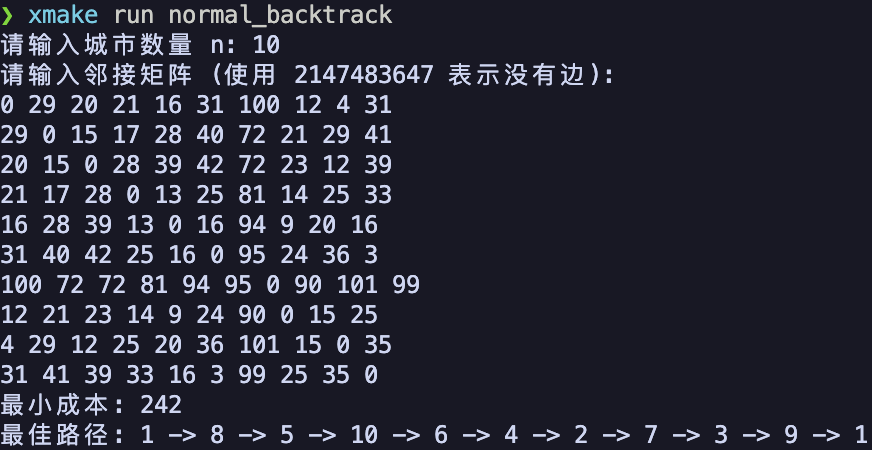
\includegraphics[width=0.8\textwidth]{images/backtrack.png}
    \caption{回溯法求解 $n=10$ 结果}
    \label{fig:backtrack}
\end{figure}
\begin{figure}[htbp]
    \centering
    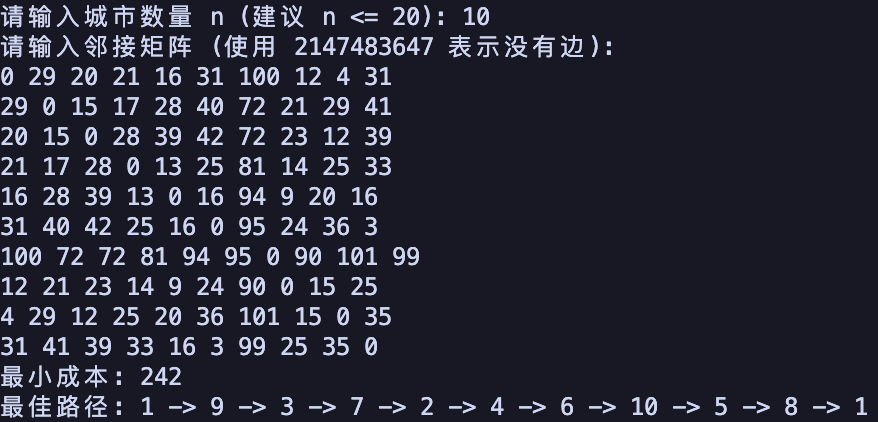
\includegraphics[width=0.8\textwidth]{images/dp.png}
    \caption{动态规划法求解 $n=10$ 结果}
    \label{fig:dp}
\end{figure}

可以看到二者给出了相同的最优值,最小成本为 242。但是给出来的路径不同,经过验证,二者均是最优解。

\subsubsection{近似算法}

分别对最近邻贪心算法、最小生成树欧拉图+最小权重匹配、对交换、模拟蚁群算法进行测试,得到结果如~\autoref{fig:nearest}、~\autoref{fig:mst}、~\autoref{fig:twoopt} 和~\autoref{fig:ant} 所示。
\begin{figure}[htbp]
    \centering
    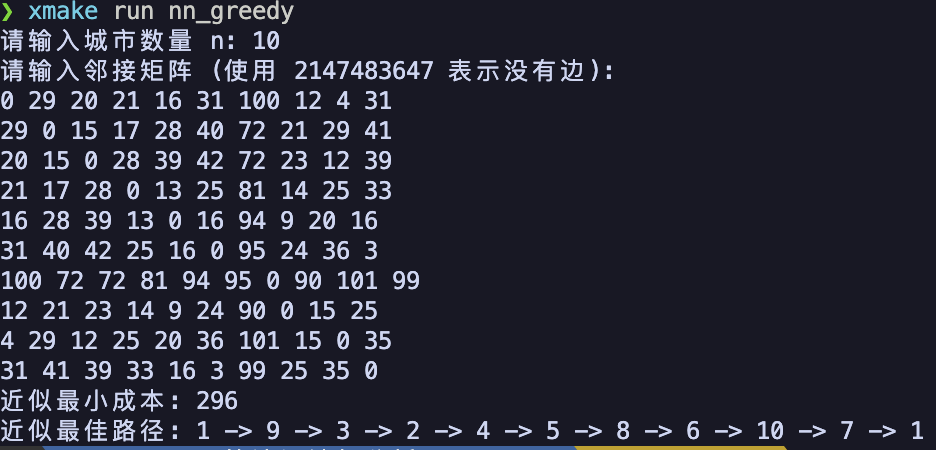
\includegraphics[width=0.8\textwidth]{images/greedy_10.png}
    \caption{最近邻贪心算法求解 $n=10$ 结果}
    \label{fig:nearest}
\end{figure}
\begin{figure}[htbp]
    \centering
    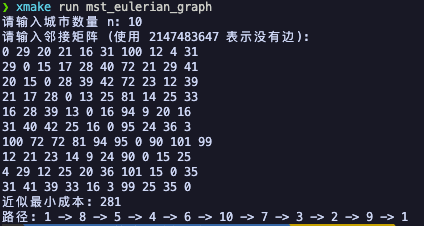
\includegraphics[width=0.8\textwidth]{images/mst_10.png}
    \caption{最小生成树欧拉图+最小权重匹配算法求解 $n=10$ 结果}
    \label{fig:mst}
\end{figure}
\begin{figure}[htbp]
    \centering
    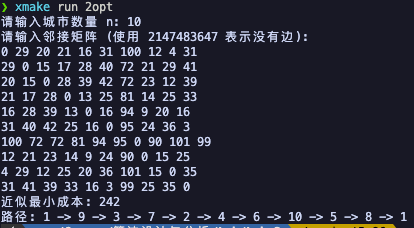
\includegraphics[width=0.8\textwidth]{images/2opt_10.png}
    \caption{对交换算法求解 $n=10$ 结果}
    \label{fig:twoopt}
\end{figure}
\begin{figure}[htbp]
    \centering
    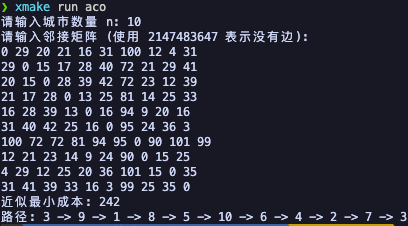
\includegraphics[width=0.8\textwidth]{images/aco_10.png}
    \caption{模拟蚁群算法求解 $n=10$ 结果}
    \label{fig:ant}
\end{figure}

得到最小成本如下:\begin{itemize}
    \item 最近邻贪心算法:296
    \item 最小生成树欧拉图+最小权重匹配:281
    \item 对交换:242
    \item 模拟蚁群算法:242
\end{itemize}

可以发现,对交换和模拟蚁群算法给出了最优解,而最近邻贪心算法和最小生成树欧拉图+最小权重匹配算法给出了次优解,但相差不算太大。

\subsection{随机生成 $n=100$}
分别对最近邻贪心算法、最小生成树欧拉图+最小权重匹配、对交换、模拟蚁群算法进行测试,得到结果如~\autoref{fig:nearest-100}、~\autoref{fig:mst-100}、~\autoref{fig:twoopt-100} 和~\autoref{fig:ant-100} 所示。
\begin{figure}[htbp]
    \centering
    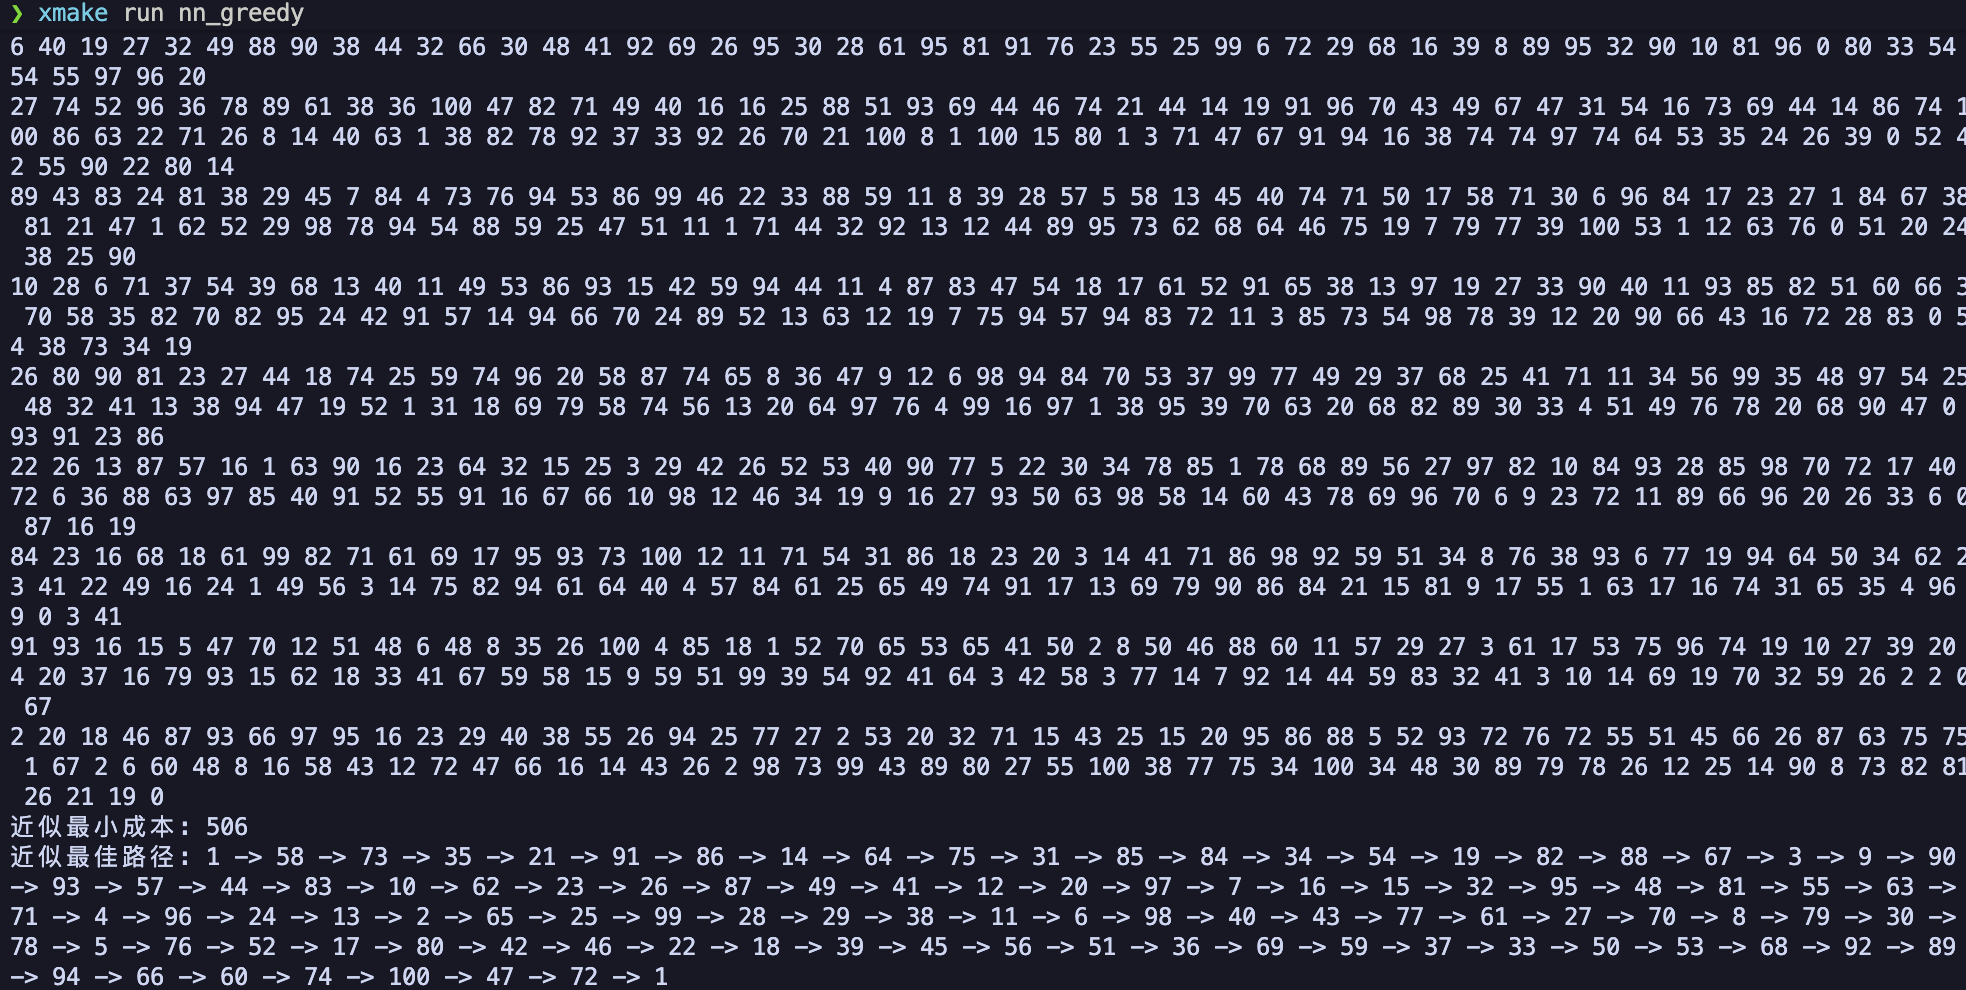
\includegraphics[width=0.8\textwidth]{images/greedy_100.png}
    \caption{最近邻贪心算法求解 $n=100$ 结果}
    \label{fig:nearest-100}
\end{figure}
\begin{figure}[htbp]
    \centering
    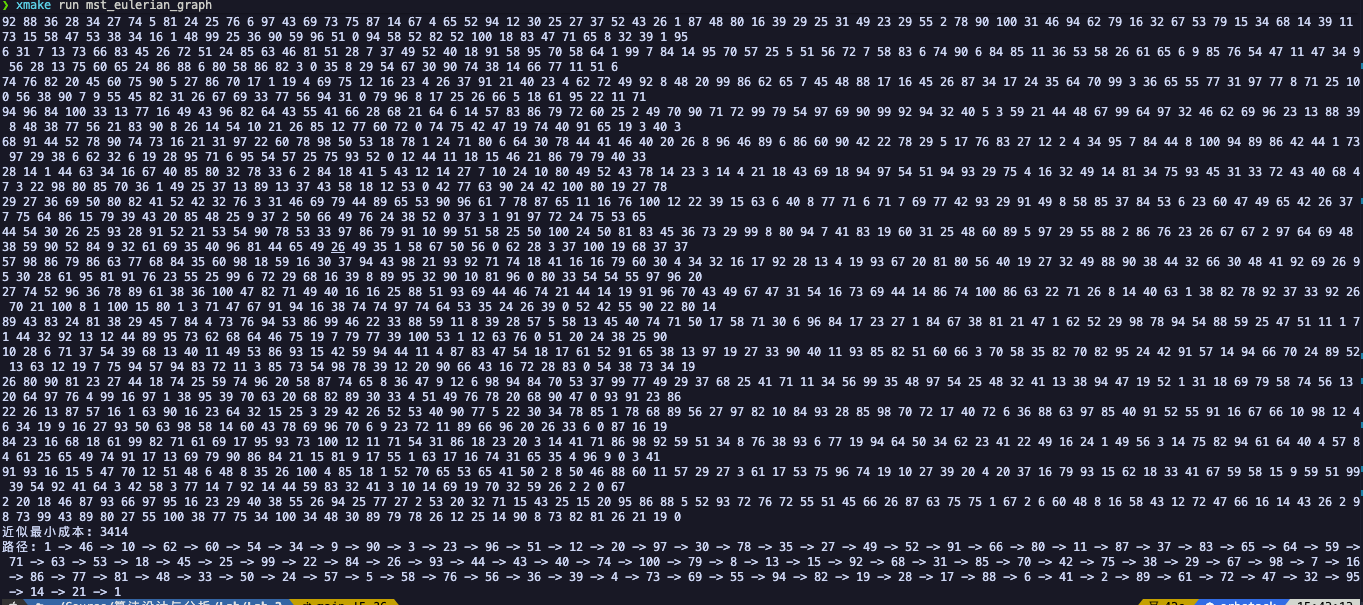
\includegraphics[width=0.8\textwidth]{images/mst_100.png}
    \caption{最小生成树欧拉图+最小权重匹配算法求解 $n=100$ 结果}
    \label{fig:mst-100}
\end{figure}
\begin{figure}[htbp]
    \centering
    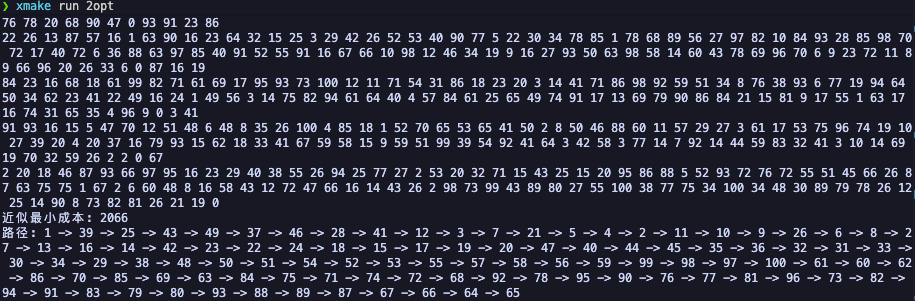
\includegraphics[width=0.8\textwidth]{images/2opt_100.png}
    \caption{对交换算法求解 $n=100$ 结果}
    \label{fig:twoopt-100}
\end{figure}
\begin{figure}[htbp]
    \centering
    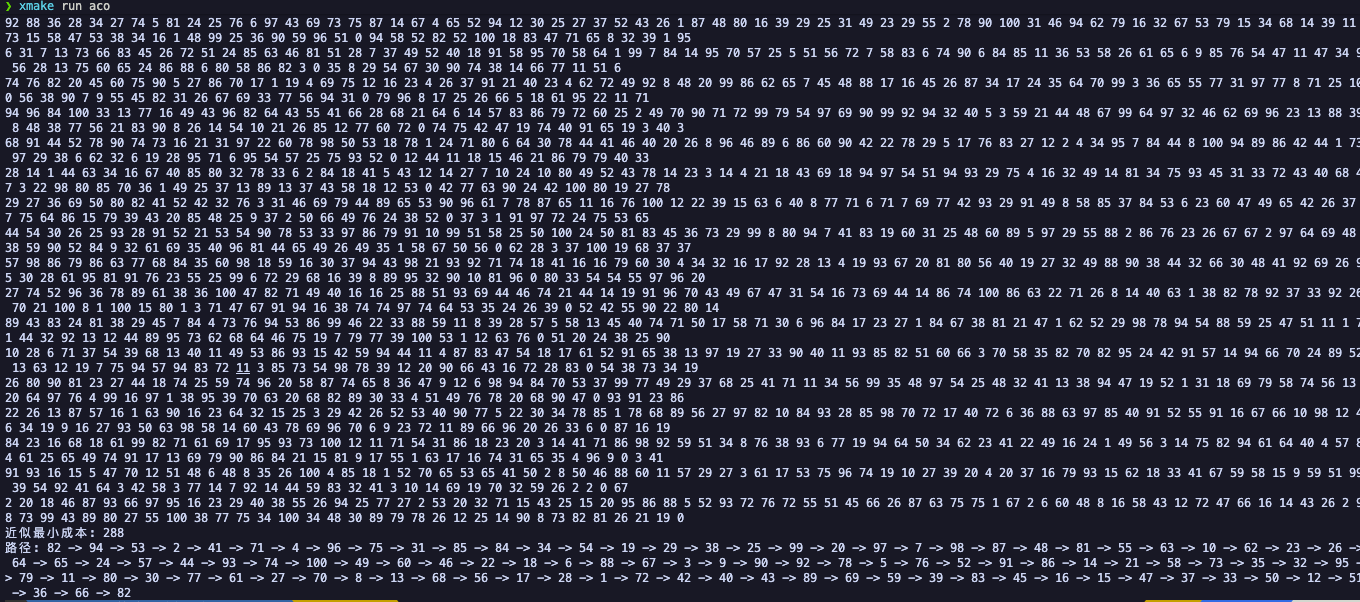
\includegraphics[width=0.8\textwidth]{images/aco_100.png}
    \caption{模拟蚁群算法求解 $n=100$ 结果}
    \label{fig:ant-100}
\end{figure}

得到最小成本如下:\begin{itemize}
    \item 最近邻贪心算法:506
    \item 最小生成树欧拉图+最小权重匹配:3414
    \item 对交换:2066
    \item 模拟蚁群算法:288
\end{itemize}

可以发现,模拟蚁群算法得益于群体智能的特性,表现仍然最出色。令人惊讶的是最近邻贪心算法的表现比剩下其他两个算法要好,其原因可能在于随机生成数据时,点之间的距离通常没有明显的模式,接近均匀分布,最近邻算法虽然是贪心策略,但在随机场景下,其结果可能已接近平均解质量。

其他算法的优化策略的核心都在于抓取路径的局部特征进行优化,更适用于城市间距离矩阵、物流配送网络等随机分布的矩阵,因此可能无法带来显著的改进,甚至可能因为过多的计算开销导致性能损失。

我们将会在后续对该发现进行进一步测试。

\subsection{修改的随机生成 $n=100$}
为了确保不是代码的问题,以及对贪心算法的缺点进行测试。我们将上一轮测试的数据稍作修改,将最近邻贪心线路终点回到起始点的代价增加 3000,进行测试。得到结果如~\autoref{fig:nearest-bad}、~\autoref{fig:mst-bad}、~\autoref{fig:twoopt-bad} 和~\autoref{fig:ant-bad} 所示。
\begin{figure}[htbp]
    \centering
    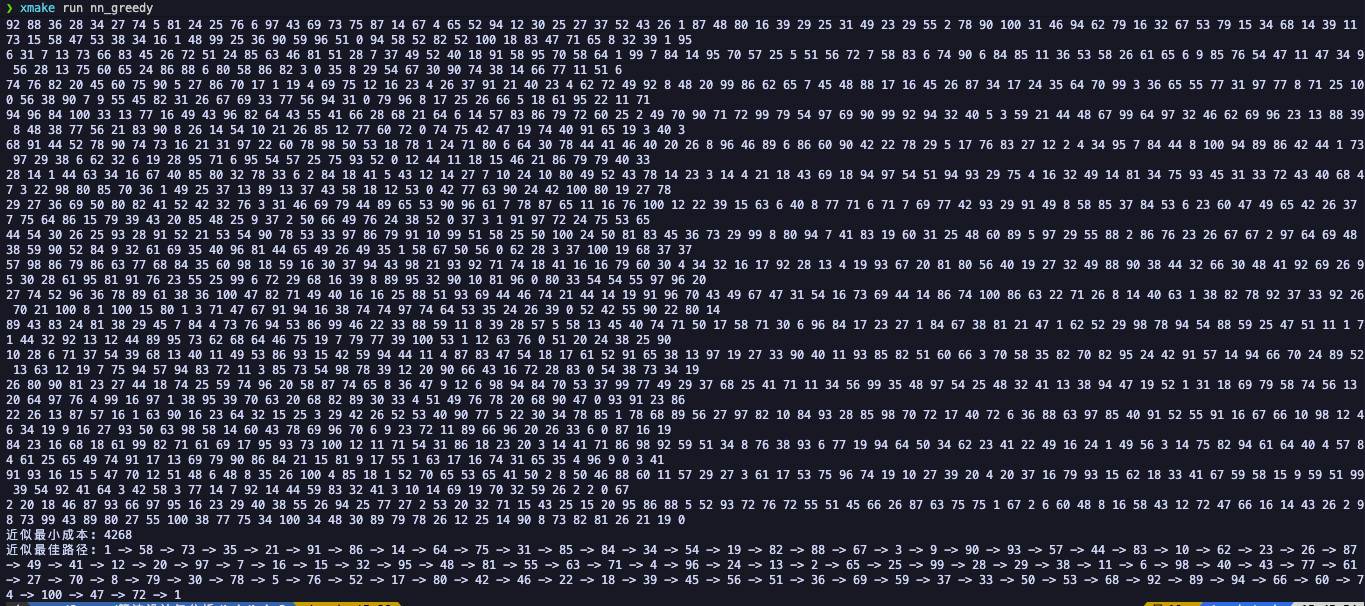
\includegraphics[width=0.8\textwidth]{images/greedy_bad.png}
    \caption{最近邻贪心算法求解修改后 $n=100$ 结果}
    \label{fig:nearest-bad}
\end{figure}
\begin{figure}[htbp]
    \centering
    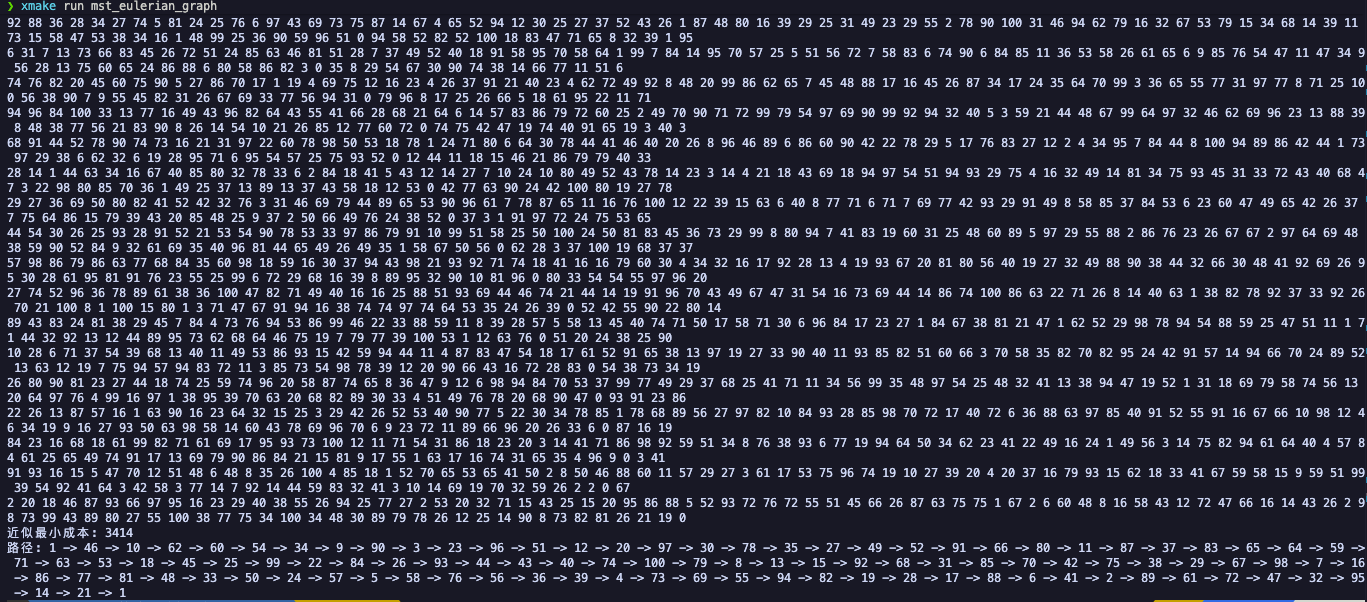
\includegraphics[width=0.8\textwidth]{images/mst_bad.png}
    \caption{最小生成树欧拉图+最小权重匹配算法求解修改后 $n=100$ 结果}
    \label{fig:mst-bad}
\end{figure}
\begin{figure}[htbp]
    \centering
    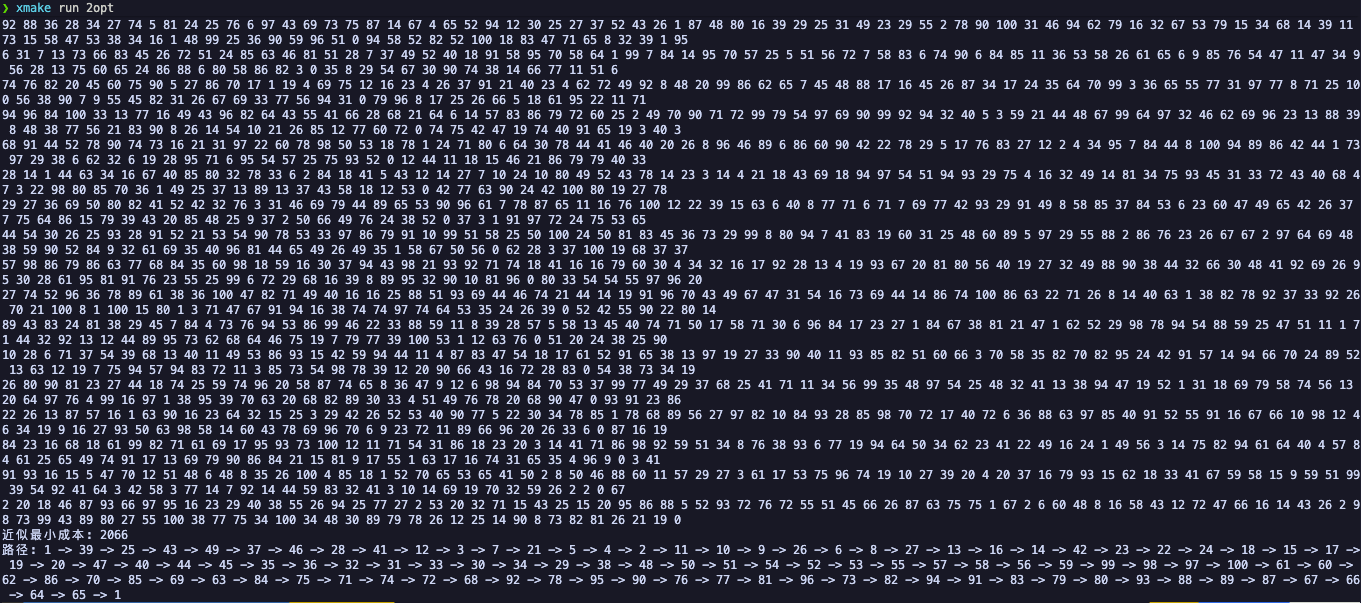
\includegraphics[width=0.8\textwidth]{images/2opt_bad.png}
    \caption{对交换算法求解修改后 $n=100$ 结果}
    \label{fig:twoopt-bad}
\end{figure}
\begin{figure}[htbp]
    \centering
    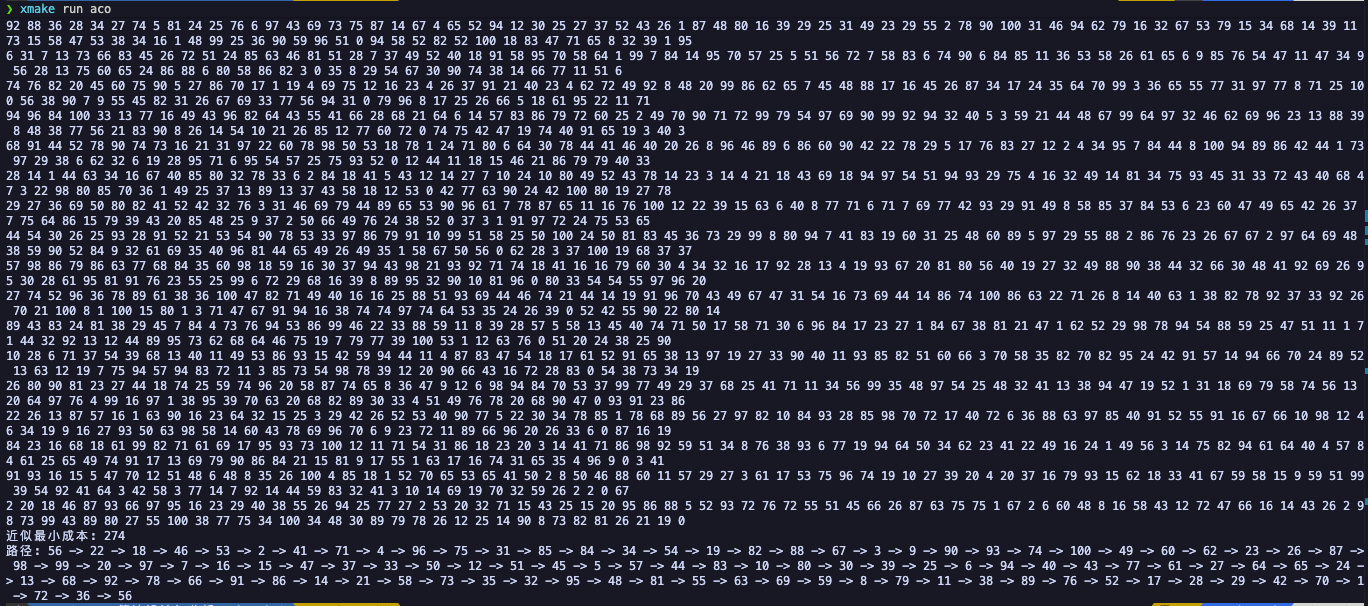
\includegraphics[width=0.8\textwidth]{images/aco_bad.png}
    \caption{模拟蚁群算法求解修改后 $n=100$ 结果}
    \label{fig:ant-bad}
\end{figure}

得到最小成本如下:\begin{itemize}
    \item 最近邻贪心算法:4268
    \item 最小生成树欧拉图+最小权重匹配:3414
    \item 对交换:2066
    \item 模拟蚁群算法:274
\end{itemize}

可以看到,贪心算法没有避开该修改,蚁群算法由于具有随机性,结果稍有不同,而其他算法仍然保持不变,避开了该不合理路径。这证明了贪心算法的局限性,以及其他算法的鲁棒性。

\subsection{实际城市数据(中国各省会距离)测试}
为了确定各种方法在实际城市数据上的表现,同时确定贪心算法此前表现优异是因为随机生成数据,我们爬取了中国各省市省会之间距离矩阵(km),作为输入进行测试。得到结果如~\autoref{fig:nearest-city}、~\autoref{fig:mst-city}、~\autoref{fig:twoopt-city} 和~\autoref{fig:ant-city} 所示。
\begin{figure}[htbp]
    \centering
    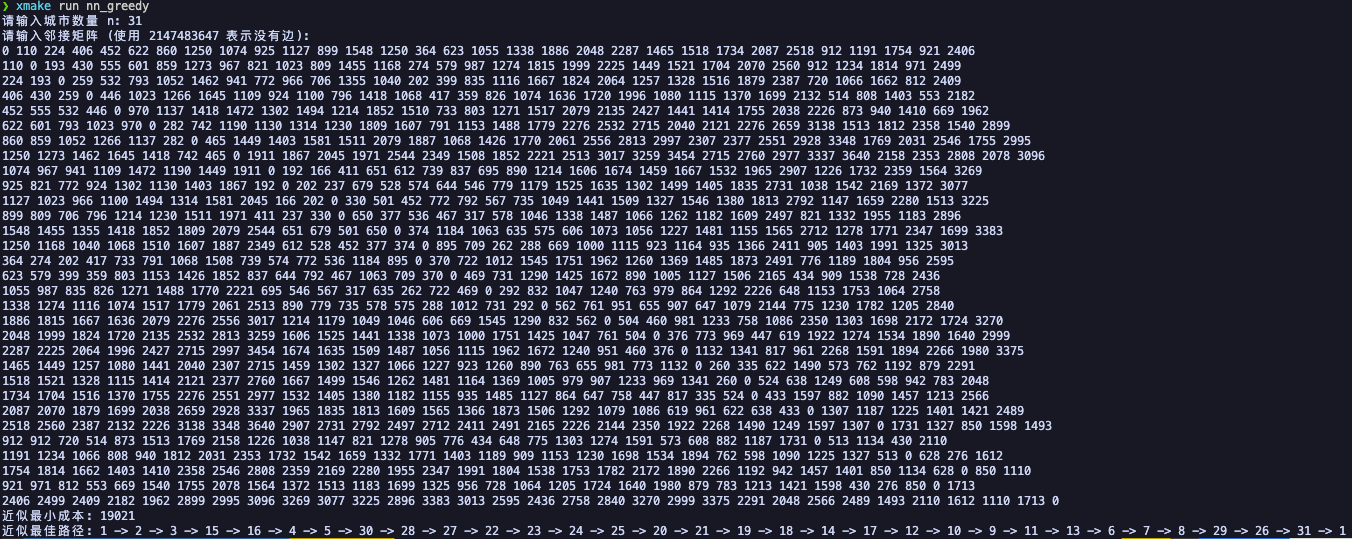
\includegraphics[width=0.8\textwidth]{images/greedy_city.png}
    \caption{最近邻贪心算法求解实际数据结果}
    \label{fig:nearest-city}
\end{figure}
\begin{figure}[htbp]
    \centering
    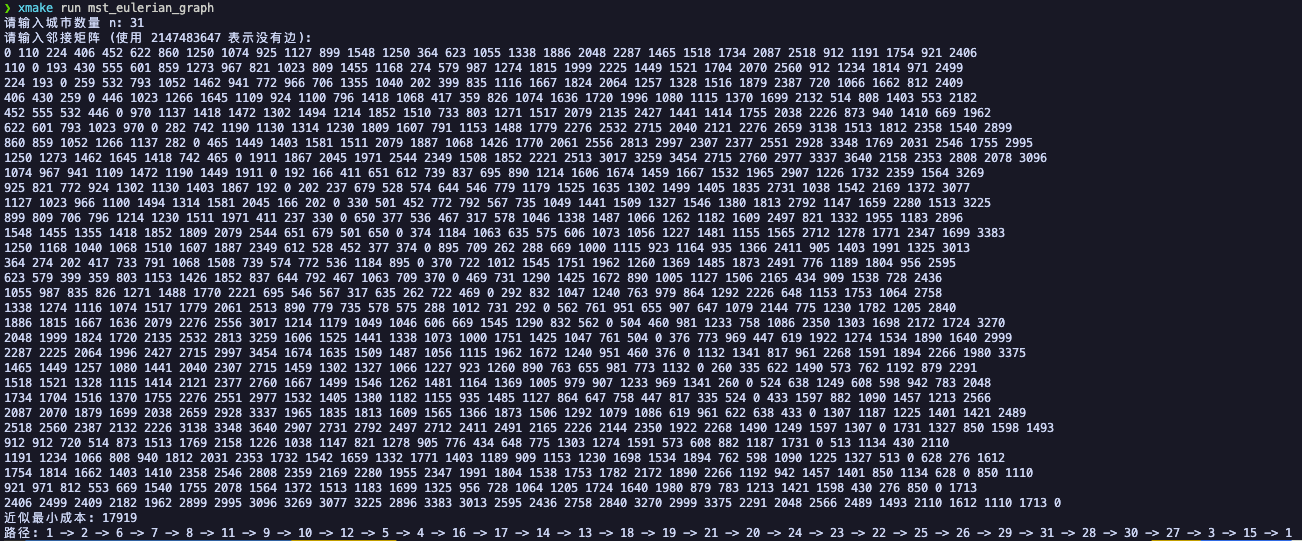
\includegraphics[width=0.8\textwidth]{images/mst_city.png}
    \caption{最小生成树欧拉图+最小权重匹配算法求解实际数据结果}
    \label{fig:mst-city}
\end{figure}
\begin{figure}[htbp]
    \centering
    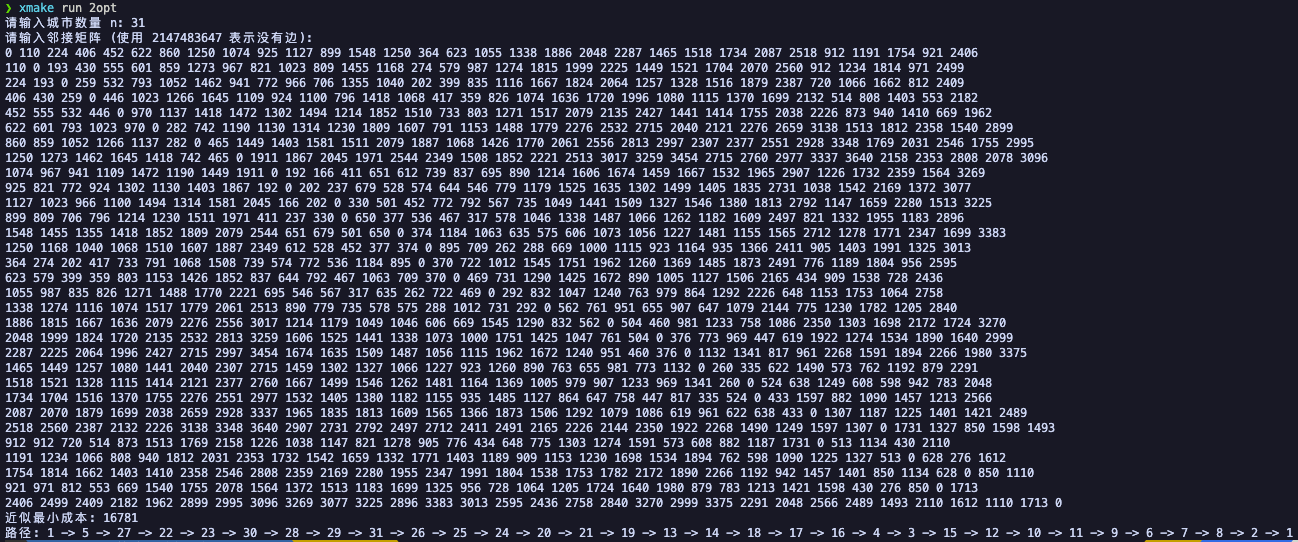
\includegraphics[width=0.8\textwidth]{images/2opt_city.png}
    \caption{对交换算法求解实际数据结果}
    \label{fig:twoopt-city}
\end{figure}
\begin{figure}[htbp]
    \centering
    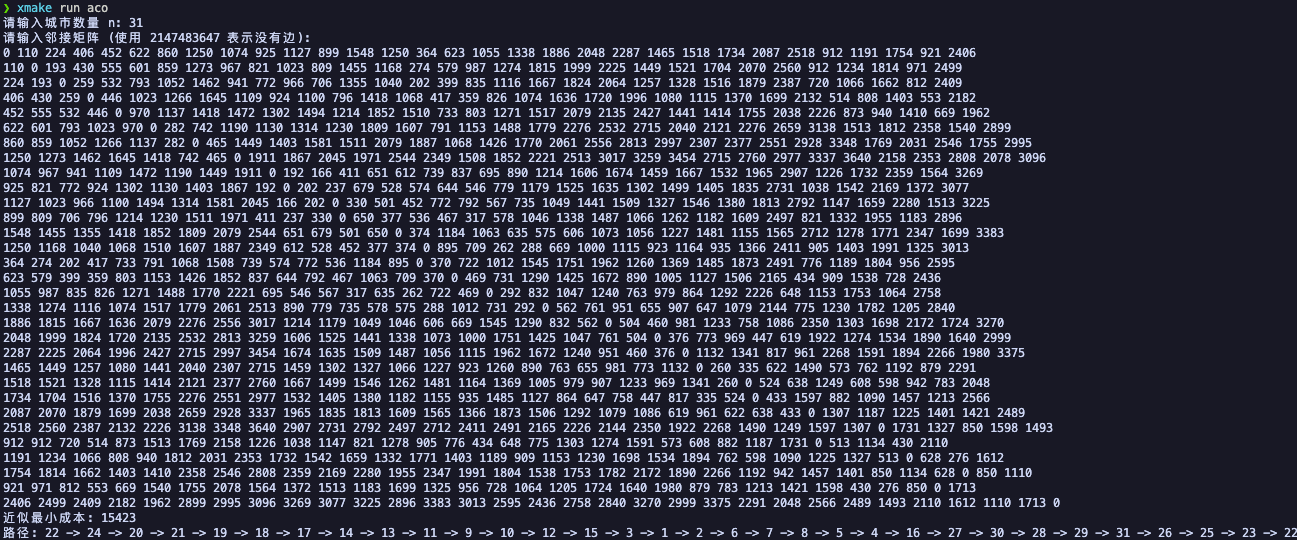
\includegraphics[width=0.8\textwidth]{images/aco_city.png}
    \caption{模拟蚁群算法求解实际数据结果}
    \label{fig:ant-city}
\end{figure}

得到最小成本如下:\begin{itemize}
    \item 最近邻贪心算法:19021
    \item 最小生成树欧拉图+最小权重匹配:17919
    \item 对交换:16781
    \item 模拟蚁群算法:15423
\end{itemize}

可以看到结果符合预期,贪心算法表现最差,模拟蚁群算法表现最好,其他算法居中。这也验证了我们的猜想,贪心算法在随机数据上表现优异,但在实际数据上表现不佳。综合表现最好的仍然为模拟蚁群算法。
\section{算法改进}

\subsection{回溯法改进}
\begin{itemize}
    \item 通过下界估计和动态更新最优解,尽早剪枝。
    \item 优先选择成本较低的边,提升找到优质解的速度。
    \item 预计算最小出边,使用位掩码表示访问状态,提升效率。
    \item 使用结构体封装状态,提升代码的可维护性和并行化能力。
\end{itemize}

但这些优化都是常数级别的优化,没有从本质上改进回溯法的时间复杂度。经过测试,仍然可以求解出最优解,实验结果如~\autoref{fig:backtrack-improved} 所示。
\begin{figure}[htbp]
    \centering
    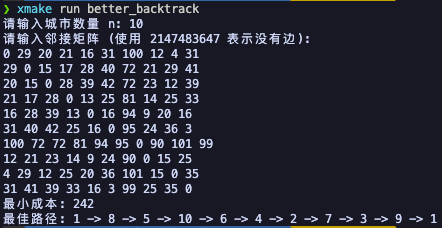
\includegraphics[width=0.8\textwidth]{images/backtrack_improved.png}
    \caption{改进后的回溯法求解 $n=10$ 结果}
    \label{fig:backtrack-improved}
\end{figure}

\subsection{动态规划法改进}
\begin{itemize}
    \item 将父节点信息存储在一个压缩的结构中,以减少空间占用。
    \item 使用结构体封装状态,提升代码的可维护性和并行化能力。
\end{itemize}

由于在实现时已经对动态规划法进行了较多的优化,因此改进的空间有限。经过测试,仍然可以求解出最优解,实验结果如~\autoref{fig:dp-improved} 所示。
\begin{figure}[htbp]
    \centering
    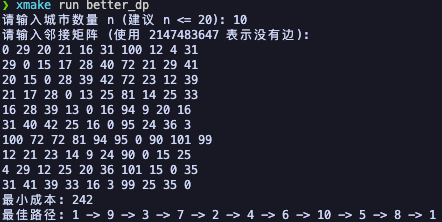
\includegraphics[width=0.8\textwidth]{images/dp_improved.png}
    \caption{改进后的动态规划法求解 $n=10$ 结果}
    \label{fig:dp-improved}
\end{figure}

\section{总结}

旅行商问题(TSP)是组合优化领域的典范问题,其研究不仅是理论算法的试炼场,更是对现实中复杂系统建模能力的严峻考验。解决TSP的过程,既是一场对优化方法的深入探索,也是一场对计算资源与算法效率极限的博弈。

在实验中,回溯法和动态规划法作为精确算法,展现了扎实的理论基础和优雅的求解思路。回溯法通过深度优先的遍历将所有可能解一一排查,结合剪枝策略尽量减少冗余计算,它展现的是一种``枚举中见智慧''的策略。而动态规划法凭借其明确的状态转移关系,将复杂问题逐层分解为子问题,利用子问题的最优性逐步合成全局最优解。这种方法让人感受到数学与算法结合的力量,但二者均未能摆脱计算复杂度随规模指数增长的困境。当面对更大规模的TSP时,这种全局最优的执念显得有些代价高昂。

相比之下,近似算法为问题的解决带来了更多灵活性与适应性。最近邻贪心算法以直观且快速的策略为特点,尽管在局部路径选择上显得轻松自如,但在全局优化上的短视属性让它在复杂或非均匀分布数据中暴露出劣势。对交换算法通过逐步调整路径结构,不断接近局部最优,展现了一种求解``局部最优的攀升之路'',但它仍需依赖良好的初始解。最小生成树结合欧拉图的策略,则以图论的严谨为基础,通过构建结构化的路径方案为问题提供了较高的解质量。而模拟蚁群算法以群体智能为特色,将自然界中蚂蚁的信息素机制引入优化问题,不仅以其强大的适应性与全局搜索能力胜出,更令人赞叹的是,它通过迭代与随机性融入了探索与利用的平衡,在实际场景中表现尤为出色。

通过不同数据集的测试,算法性能的差异逐渐显现。精确算法在小规模问题上提供了参考标准,而近似算法在大规模和现实数据中的优劣则依次揭示。在随机生成的数据中,最近邻贪心算法意外表现出较好的竞争力,这可能是由于数据分布的均匀性使得其局限性被弱化。然而,在经过特定修改的数据和实际城市间距离矩阵中,其缺陷暴露无遗。而模拟蚁群算法则凭借其自适应性和群体协作的优势,在各种场景下始终表现优异,显示了其作为高效启发式方法的独特潜力。

这一系列实验不仅让我们体会到算法间性能的优劣,更加深了对优化方法本质的理解。每一种算法,都反映了其背后设计思想的局限与可能性;每一种表现,都诉说了问题结构与求解策略间的深刻联系。TSP问题的研究,不仅是为了找到某个问题的最优解,更在于通过这一过程,探究优化的原理、模型的特性以及解决复杂问题的多样化路径。正是这种对问题的深入思考与实践,让TSP超越了一个单纯的学术课题,成为我们理解优化科学与系统复杂性的一个经典窗口。

\newpage

\printbibliography

\newpage

\appendix

\section{关键源码}

\textcolor{red}{注:虽然本报告参考了一些论文,但关键源码均为自己实现。}

\subsection{回溯法}

\begin{cppcode}
const int NoEdge = INT32_MAX;

int bestc = NoEdge;
std::vector<int> bestx;
int cc = 0;

void Backtrack(int i, int n, const std::vector<std::vector<int>> &a, std::vector<int> &x) {
    if (i == n) {
        if (a[x[n - 1]][x[n]] != NoEdge && a[x[n]][0] != NoEdge) {
            int totalCost = cc + a[x[n - 1]][x[n]] + a[x[n]][0];
            if (totalCost < bestc || bestc == NoEdge) {
                bestc = totalCost;
                // Update the best path
                for (int j = 0; j <= n; ++j) {
                    bestx[j] = x[j];
                }
            }
        }
    } else {
        for (int j = i; j <= n; ++j) {
            if (a[x[i - 1]][x[j]] != NoEdge &&
                (cc + a[x[i - 1]][x[j]] < bestc || bestc == NoEdge)) {
                std::swap(x[i], x[j]);
                cc += a[x[i - 1]][x[i]];
                Backtrack(i + 1, n, a, x);
                cc -= a[x[i - 1]][x[i]];
                std::swap(x[i], x[j]); // backtrack
            }
        }
    }
}

int TSP(const std::vector<std::vector<int>> &a, std::vector<int> &v, int n) {
    std::vector<int> x(n + 1);
    for (int i = 0; i <= n; ++i) {
        x[i] = i;
    }

    bestx.assign(n + 1, 0);
    for (int i = 0; i <= n; ++i) {
        bestx[i] = x[i];
    }

    Backtrack(1, n, a, x);

    for (int i = 0; i <= n; ++i) {
        v[i] = bestx[i];
    }

    return bestc;
}
\end{cppcode}

\subsection{动态规划}

\begin{cppcode}
const int NoEdge = INT32_MAX;

std::vector<int> ReconstructPath(const std::vector<std::vector<int>> &parent, int final_mask, int last_city, int n) {
    std::vector<int> path;
    
    int mask = final_mask;
    int current_city = last_city;

    while (current_city != 0) {
        path.push_back(current_city);
        int prev_city = parent[mask][current_city];
        mask &= ~(1 << current_city);
        current_city = prev_city;
    }

    path.push_back(0);

    std::reverse(path.begin(), path.end());

    path.push_back(0);

    return path;
}

int TSP_DP(const std::vector<std::vector<int>> &a, int n, std::vector<int> &bestx) {
    int N = 1 << n;
    std::vector<std::vector<int>> dp(N, std::vector<int>(n, NoEdge));
    std::vector<std::vector<int>> parent(N, std::vector<int>(n, -1));

    dp[1][0] = 0;

    for (int mask = 1; mask < N; ++mask) {
        for (int u = 0; u < n; ++u) {
            if (mask & (1 << u)) {
                if (dp[mask][u] == NoEdge) continue;

                for (int v = 0; v < n; ++v) {
                    if (!(mask & (1 << v)) && a[u][v] != NoEdge) {
                        int next_mask = mask | (1 << v);
                        if (dp[next_mask][v] > dp[mask][u] + a[u][v]) {
                            dp[next_mask][v] = dp[mask][u] + a[u][v];
                            parent[next_mask][v] = u;
                        }
                    }
                }
            }
        }
    }

    int final_mask = N - 1; 
    int min_cost = NoEdge;
    int last_city = -1;

    for (int u = 1; u < n; ++u) {
        if (a[u][0] != NoEdge && dp[final_mask][u] != NoEdge) {
            int total_cost = dp[final_mask][u] + a[u][0];
            if (total_cost < min_cost) {
                min_cost = total_cost;
                last_city = u;
            }
        }
    }

    if (min_cost == NoEdge) {
        return NoEdge;
    }

    bestx = ReconstructPath(parent, final_mask, last_city, n);

    return min_cost;
}
\end{cppcode}

\subsection{最近邻贪心算法}

\begin{cppcode}
bool NearestNeighbor(const std::vector<std::vector<int>> &adj, int n, std::vector<int> &path, int &totalCost) {
    if (n == 0) return false;

    std::vector<bool> visited(n, false);
    path.clear();
    totalCost = 0;

    int currentCity = 0;
    path.push_back(currentCity);
    visited[currentCity] = true;

    for (int step = 1; step < n; ++step) {
        int nearestCity = -1;
        int minCost = NoEdge;

        for (int city = 0; city < n; ++city) {
            if (!visited[city] && adj[currentCity][city] < minCost && city != currentCity) {
                minCost = adj[currentCity][city];
                nearestCity = city;
            }
        }

        if (nearestCity == -1 || minCost == NoEdge) {
            return false;
        }

        path.push_back(nearestCity);
        visited[nearestCity] = true;
        totalCost += minCost;
        currentCity = nearestCity;
    }

    if (adj[currentCity][path[0]] == NoEdge) {
        return false;
    }
    path.push_back(path[0]);
    totalCost += adj[currentCity][path[0]];

    return true;
}
\end{cppcode}

\subsection{最小生成树欧拉图 + 最小权重匹配}

\begin{cppcode}
const int NoEdge = INT32_MAX;

struct Edge {
    int u, v, weight;
    bool operator<(const Edge &other) const {
        return weight < other.weight;
    }
};

std::vector<Edge> FindMST(const std::vector<std::vector<int>> &graph, int n) {
    std::vector<Edge> edges;
    for (int u = 0; u < n; ++u) {
        for (int v = u + 1; v < n; ++v) {
            if (graph[u][v] != NoEdge) {
                edges.push_back({u, v, graph[u][v]});
            }
        }
    }

    std::sort(edges.begin(), edges.end());

    std::vector<int> parent(n);
    for (int i = 0; i < n; ++i) {
        parent[i] = i;
    }

    auto Find = [&](int x) -> int {
        while (x != parent[x]) {
            parent[x] = parent[parent[x]];
            x = parent[x];
        }
        return x;
    };

    auto Union = [&](int x, int y) {
        parent[Find(x)] = Find(y);
    };

    std::vector<Edge> mst;
    for (const Edge &e : edges) {
        if (Find(e.u) != Find(e.v)) {
            mst.push_back(e);
            Union(e.u, e.v);
            if (mst.size() == n - 1) {
                break;
            }
        }
    }

    return mst;
}

std::vector<int> FindOddVertices(const std::vector<Edge> &mst, int n) {
    std::vector<int> degree(n, 0);
    for (const Edge &e : mst) {
        degree[e.u]++;
        degree[e.v]++;
    }

    std::vector<int> oddVertices;
    for (int i = 0; i < n; ++i) {
        if (degree[i] % 2 == 1) {
            oddVertices.push_back(i);
        }
    }

    return oddVertices;
}

std::vector<Edge> FindMinimumPerfectMatching(const std::vector<int> &oddVertices,
                                             const std::vector<std::vector<int>> &graph) {
    std::vector<Edge> matching;
    std::set<int> unmatched(oddVertices.begin(), oddVertices.end());

    while (!unmatched.empty()) {
        int u = *unmatched.begin();
        unmatched.erase(u);

        int minWeight = INT32_MAX;
        int bestMatch = -1;

        for (int v : unmatched) {
            if (graph[u][v] < minWeight) {
                minWeight = graph[u][v];
                bestMatch = v;
            }
        }

        if (bestMatch != -1) {
            unmatched.erase(bestMatch);
            matching.push_back({u, bestMatch, minWeight});
        } else {
        }
    }

    return matching;
}

std::vector<int> FindEulerianTour(const std::vector<Edge> &mst,
                                  const std::vector<Edge> &matching, int n) {
    std::vector<std::vector<int>> adjList(n, std::vector<int>());
    for (const Edge &e : mst) {
        adjList[e.u].push_back(e.v);
        adjList[e.v].push_back(e.u);
    }
    for (const Edge &e : matching) {
        adjList[e.u].push_back(e.v);
        adjList[e.v].push_back(e.u);
    }

    std::vector<int> tour;
    std::vector<std::vector<int>> localAdj = adjList;

    std::function<void(int)> Hierholzer = [&](int u) {
        while (!localAdj[u].empty()) {
            int v = localAdj[u].back();
            localAdj[u].pop_back();
            auto &vec = localAdj[v];
            vec.erase(std::find(vec.begin(), vec.end(), u));
            Hierholzer(v);
        }
        tour.push_back(u);
    };

    Hierholzer(0);
    std::reverse(tour.begin(), tour.end());
    return tour;
}

std::vector<int> CompressEulerianToHamiltonian(const std::vector<int> &eulerTour) {
    std::vector<int> hamiltonian;
    std::set<int> visited;
    for (int city : eulerTour) {
        if (visited.find(city) == visited.end()) {
            visited.insert(city);
            hamiltonian.push_back(city);
        }
    }
    return hamiltonian;
}

std::pair<int, std::vector<int>> GetMSTBasedTSP(const std::vector<std::vector<int>> &graph, int n) {
    std::vector<Edge> mst = FindMST(graph, n);

    std::vector<int> oddVertices = FindOddVertices(mst, n);

    std::vector<Edge> matching = FindMinimumPerfectMatching(oddVertices, graph);

    std::vector<int> eulerTour = FindEulerianTour(mst, matching, n);

    std::vector<int> hamiltonianPath = CompressEulerianToHamiltonian(eulerTour);

    if (!hamiltonianPath.empty()) {
        hamiltonianPath.push_back(hamiltonianPath[0]);
    }

    int totalCost = 0;
    for (size_t i = 0; i < hamiltonianPath.size() - 1; ++i) {
        int from = hamiltonianPath[i];
        int to = hamiltonianPath[i + 1];
        if (graph[from][to] == NoEdge) {
        }
        totalCost += graph[from][to];
    }

    return {totalCost, hamiltonianPath};
}
\end{cppcode}

\subsection{对交换}

\begin{cppcode}
const int NoEdge = std::numeric_limits<int>::max();

int CalculatePathCost(const std::vector<int> &path, const std::vector<std::vector<int>> &adj) {
    int cost = 0;
    int n = path.size();
    for (int i = 0; i < n - 1; ++i) {
        cost += adj[path[i]][path[i + 1]];
    }
    cost += adj[path.back()][path[0]];
    return cost;
}

std::vector<int> TwoOptSwap(const std::vector<int> &path, int i, int k) {
    std::vector<int> newPath;
    newPath.insert(newPath.end(), path.begin(), path.begin() + i);
    std::vector<int> reversedSegment(path.begin() + i, path.begin() + k + 1);
    std::reverse(reversedSegment.begin(), reversedSegment.end());
    newPath.insert(newPath.end(), reversedSegment.begin(), reversedSegment.end());
    newPath.insert(newPath.end(), path.begin() + k + 1, path.end());
    return newPath;
}

std::pair<int, std::vector<int>> TwoOpt(const std::vector<std::vector<int>> &graph, const std::vector<int> &initialPath) {
    int n = initialPath.size();
    std::vector<int> bestPath = initialPath;
    int bestCost = CalculatePathCost(bestPath, graph);

    bool improvement = true;
    while (improvement) {
        improvement = false;
        for (int i = 1; i < n - 1; ++i) {
            for (int k = i + 1; k < n; ++k) {
                std::vector<int> newPath = TwoOptSwap(bestPath, i, k);
                int newCost = CalculatePathCost(newPath, graph);
                if (newCost < bestCost) {
                    bestPath = newPath;
                    bestCost = newCost;
                    improvement = true;
                }
            }
        }
    }

    return {bestCost, bestPath};
}
\end{cppcode}

\subsection{模拟蚁群算法(ACS)}
\begin{cppcode}
const int NoEdge = std::numeric_limits<int>::max();
const double alpha = 1.0; // 信息素重要程度
const double beta = 5.0;  // 启发式信息重要程度
const double rho = 0.5;   // 信息素挥发系数
const double Q = 100.0;   // 常数用于信息素更新
const int MAX_ITER = 1000; // 最大迭代次数
const int NUM_ANTS = 20;   // 蚂蚁数量

int CalculatePathCost(const std::vector<int> &path, const std::vector<std::vector<int>> &adj) {
    int cost = 0;
    int n = path.size();
    for (int i = 0; i < n - 1; ++i) {
        cost += adj[path[i]][path[i + 1]];
    }
    cost += adj[path.back()][path[0]];
    return cost;
}

int SelectNextCity(int currentCity, const std::vector<std::vector<double>> &pheromone,
                   const std::vector<std::vector<int>> &adj, const std::vector<std::vector<double>> &visibility,
                   const std::vector<bool> &visited) {
    double sumProb = 0.0;
    int n = adj.size();
    std::vector<double> prob(n, 0.0);

    for (int i = 0; i < n; ++i) {
        if (!visited[i] && adj[currentCity][i] != NoEdge) {
            prob[i] = pow(pheromone[currentCity][i], alpha) * pow(visibility[currentCity][i], beta);
            sumProb += prob[i];
        }
    }

    if (sumProb == 0) return -1;

    double randVal = ((double)rand() / RAND_MAX) * sumProb;
    double cumSum = 0.0;

    for (int i = 0; i < n; ++i) {
        if (!visited[i] && adj[currentCity][i] != NoEdge) {
            cumSum += prob[i];
            if (cumSum >= randVal) return i;
        }
    }

    return -1;
}

void UpdatePheromone(std::vector<std::vector<double>> &pheromone, const std::vector<std::vector<int>> &adj,
                     const std::vector<std::vector<int>> &antPaths, const std::vector<int> &pathCosts) {
    int n = adj.size();

    for (int i = 0; i < n; ++i) {
        for (int j = 0; j < n; ++j) {
            pheromone[i][j] *= (1.0 - rho);
        }
    }

    for (size_t ant = 0; ant < antPaths.size(); ++ant) {
        int pathCost = pathCosts[ant];
        for (size_t i = 0; i < antPaths[ant].size() - 1; ++i) {
            int from = antPaths[ant][i];
            int to = antPaths[ant][i + 1];
            pheromone[from][to] += Q / pathCost;
            pheromone[to][from] += Q / pathCost;
        }
    }
}

std::pair<int, std::vector<int>> AntColonyOptimization(const std::vector<std::vector<int>> &graph) {
    int n = graph.size();
    std::vector<std::vector<double>> pheromone(n, std::vector<double>(n, 1.0));
    std::vector<std::vector<double>> visibility(n, std::vector<double>(n, 0.0));

    for (int i = 0; i < n; ++i) {
        for (int j = 0; j < n; ++j) {
            if (graph[i][j] != NoEdge) {
                visibility[i][j] = 1.0 / graph[i][j];
            }
        }
    }

    std::vector<int> bestPath;
    int bestCost = NoEdge;
    srand(time(0)); 

    for (int iter = 0; iter < MAX_ITER; ++iter) {
        std::vector<std::vector<int>> antPaths(NUM_ANTS, std::vector<int>(n));
        std::vector<int> pathCosts(NUM_ANTS, 0);

        for (int ant = 0; ant < NUM_ANTS; ++ant) {
            std::vector<bool> visited(n, false);
            int currentCity = rand() % n;
            visited[currentCity] = true;
            antPaths[ant][0] = currentCity;

            for (int step = 1; step < n; ++step) {
                int nextCity = SelectNextCity(currentCity, pheromone, graph, visibility, visited);
                antPaths[ant][step] = nextCity;
                visited[nextCity] = true;
                currentCity = nextCity;
            }

            antPaths[ant].push_back(antPaths[ant][0]);

            pathCosts[ant] = CalculatePathCost(antPaths[ant], graph);
        }

        UpdatePheromone(pheromone, graph, antPaths, pathCosts);

        for (int ant = 0; ant < NUM_ANTS; ++ant) {
            if (pathCosts[ant] < bestCost) {
                bestCost = pathCosts[ant];
                bestPath = antPaths[ant];
            }
        }
    }

    return {bestCost, bestPath};
}    
\end{cppcode}

\subsection{改进的回溯法}

\begin{cppcode}
const int NoEdge = std::numeric_limits<int>::max();

struct TSP_Solver {
    int bestc;                      // 最佳成本
    std::vector<int> bestx;         // 最佳路径
    int cc;                         // 当前路径成本
    std::vector<int> min_out;       // 每个城市的最小出边成本

    TSP_Solver(int n) : bestc(NoEdge), bestx(n, 0), cc(0), min_out(n, NoEdge) {}

    void precompute_min_out(int n, const std::vector<std::vector<int>> &a){
        for(int i = 0; i < n; ++i){
            for(int j = 0; j < n; ++j){
                if(i != j && a[i][j] < min_out[i]){
                    min_out[i] = a[i][j];
                }
            }
        }
    }

    void Backtrack(int i, int n, const std::vector<std::vector<int>> &a, std::vector<int> &x, int visited) {
        if(i == n){
            // 检查是否可以回到起点
            if(a[x[n - 1]][x[0]] != NoEdge){
                int totalCost = cc + a[x[n - 1]][x[0]];
                if(totalCost < bestc){
                    bestc = totalCost;
                    bestx = x;
                }
            }
            return;
        }

        for(int j = 0; j < n; ++j){
            if(!(visited & (1 << j)) && a[x[i - 1]][j] != NoEdge){
                int new_cost = cc + a[x[i - 1]][j];

                // 计算下界
                int lower_bound = new_cost;
                for(int k = 0; k < n; ++k){
                    if(!(visited & (1 << k))){
                        lower_bound += min_out[k];
                    }
                }

                if(lower_bound < bestc){
                    x[i] = j;
                    cc += a[x[i - 1]][j];           
                    Backtrack(i + 1, n, a, x, visited | (1 << j)); 
                    cc -= a[x[i - 1]][j];           
                }
            }
        }
    }

    int solve(const std::vector<std::vector<int>> &a, std::vector<int> &v, int n){
        std::vector<int> x(n, 0); 
        for(int i = 0; i < n; ++i){
            x[i] = i;
        }

        bestx = x;
        precompute_min_out(n, a); 
        Backtrack(1, n, a, x, 1 << 0);

        v = bestx; 
        return bestc;
    }
};
\end{cppcode}

\subsection{改进的动态规划}
\begin{cppcode}
const int NoEdge = std::numeric_limits<int>::max();

struct TSP_Solver {
    int n; // 城市数量
    std::vector<std::vector<int>> adj; // 邻接矩阵
    std::vector<std::vector<int>> dp; // DP表
    std::vector<std::vector<int>> parent; // 父节点信息,用于路径重建

    TSP_Solver(int num_cities, const std::vector<std::vector<int>> &adj_matrix)
        : n(num_cities), adj(adj_matrix),
          dp(1 << num_cities, std::vector<int>(num_cities, NoEdge)),
          parent(1 << num_cities, std::vector<int>(num_cities, -1)) {}

    std::vector<int> ReconstructPath(int final_mask, int last_city) const {
        std::vector<int> path;
        int mask = final_mask;
        int current_city = last_city;

        while (current_city != 0) { 
            path.push_back(current_city);
            int prev_city = parent[mask][current_city];
            if (prev_city == -1) {
                return {};
            }
            mask ^= (1 << current_city);
            current_city = prev_city;
        }

        path.push_back(0);
        std::reverse(path.begin(), path.end());
        path.push_back(0); 

        return path;
    }

    int Solve(std::vector<int> &bestx) {
        dp[1 << 0][0] = 0;

        int N = 1 << n; 
        for (int mask = 1; mask < N; ++mask) {
            for (int u = 0; u < n; ++u) {
                if (!(mask & (1 << u))) continue;

                if (dp[mask][u] == NoEdge) continue;

                for (int v = 0; v < n; ++v) {
                    if (mask & (1 << v)) continue;
                    if (adj[u][v] == NoEdge) continue;

                    int next_mask = mask | (1 << v);
                    if (dp[next_mask][v] > dp[mask][u] + adj[u][v]) {
                        dp[next_mask][v] = dp[mask][u] + adj[u][v];
                        parent[next_mask][v] = u;
                    }
                }
            }
        }

        int final_mask = N - 1;
        int min_cost = NoEdge;
        int last_city = -1;

        for (int u = 1; u < n; ++u) {
            if (adj[u][0] != NoEdge && dp[final_mask][u] != NoEdge) {
                int total_cost = dp[final_mask][u] + adj[u][0];
                if (total_cost < min_cost) {
                    min_cost = total_cost;
                    last_city = u;
                }
            }
        }

        if (min_cost == NoEdge) {
            return NoEdge;
        }

        bestx = ReconstructPath(final_mask, last_city);
        return min_cost;
    }
};
\end{cppcode}